\documentclass[a4paper,12pt, twoside]{memoir}   	% use "amsart" instead of "article" for AMSLaTeX format
\usepackage{geometry}                		% See geometry.pdf to learn the layout options. There are lots.
%% \geometry{letterpaper}                   		% ... or a4paper or a5paper or ...
\geometry{vmargin=3cm}%% hmargin=2cm
\usepackage{graphicx}
\usepackage{color}
\usepackage[dvipsnames]{xcolor}
\usepackage{enumerate}
\usepackage{amssymb}
\usepackage{footnote}
\usepackage{enumerate}
\usepackage{eucal}
\usepackage{amsmath}
\usepackage{braket}
\usepackage[utf8]{inputenc}
\usepackage[english]{babel}
\usepackage{hyperref}
\usepackage{xspace}
\usepackage{pdfpages}
\usepackage{subcaption}
\usepackage[margin=2cm]{caption}
%% pour empêcher la cesure des mots
\pretolerance=10000
\tolerance=1000
\emergencystretch=10pt

\captionsetup[figure]{font=footnotesize}
\captionsetup[subfigure]{font=footnotesize}

\hypersetup{
    colorlinks,
    citecolor=red,
    filecolor=red,
    linkcolor=red,
    urlcolor=red
}

\setcounter{tocdepth}{3}
\setcounter{secnumdepth}{3}

\newcommand{\zeronu}{0\nu\beta\beta}
\newcommand{\twonu}{2\nu\beta\beta}
\newcommand{\Tl}{$^{208}$Tl}
\newcommand{\Co}{$^{60}$Co}
\newcommand{\Pb}{$^{208}$Pb}
\newcommand{\Bi}{$^{214}$Bi}
\newcommand{\Qbb}{Q_{\beta\beta}}
\newcommand{\Bckunit}{\text{counts.keV}^{-1}\text{.kg}^{-1}\text{.y}^{-1}}
\newcommand{\Tbeta}{T_{1/2}^{0\nu}}
\newcommand{\mbb}{m_{\beta\beta}}

\newcommand\myshade{85}
\colorlet{mylinkcolor}{violet}
\colorlet{mycitecolor}{YellowOrange}
\colorlet{myurlcolor}{Aquamarine}
\usepackage{hyperref} %backref
\hypersetup{
  linkcolor  = mylinkcolor!\myshade!black,
  citecolor  = mycitecolor!\myshade!black,
  urlcolor   = myurlcolor!\myshade!black,
  colorlinks = true,
}

\newenvironment{itemize*}%
  {\begin{itemize}%
    \setlength{\itemsep}{0pt}%
    %\setlength{\parskip}{0pt}
  }%
  {\end{itemize}}


%\title{}

\includeonly{commissioning/commissioning}

\begin{document}
%\maketitle
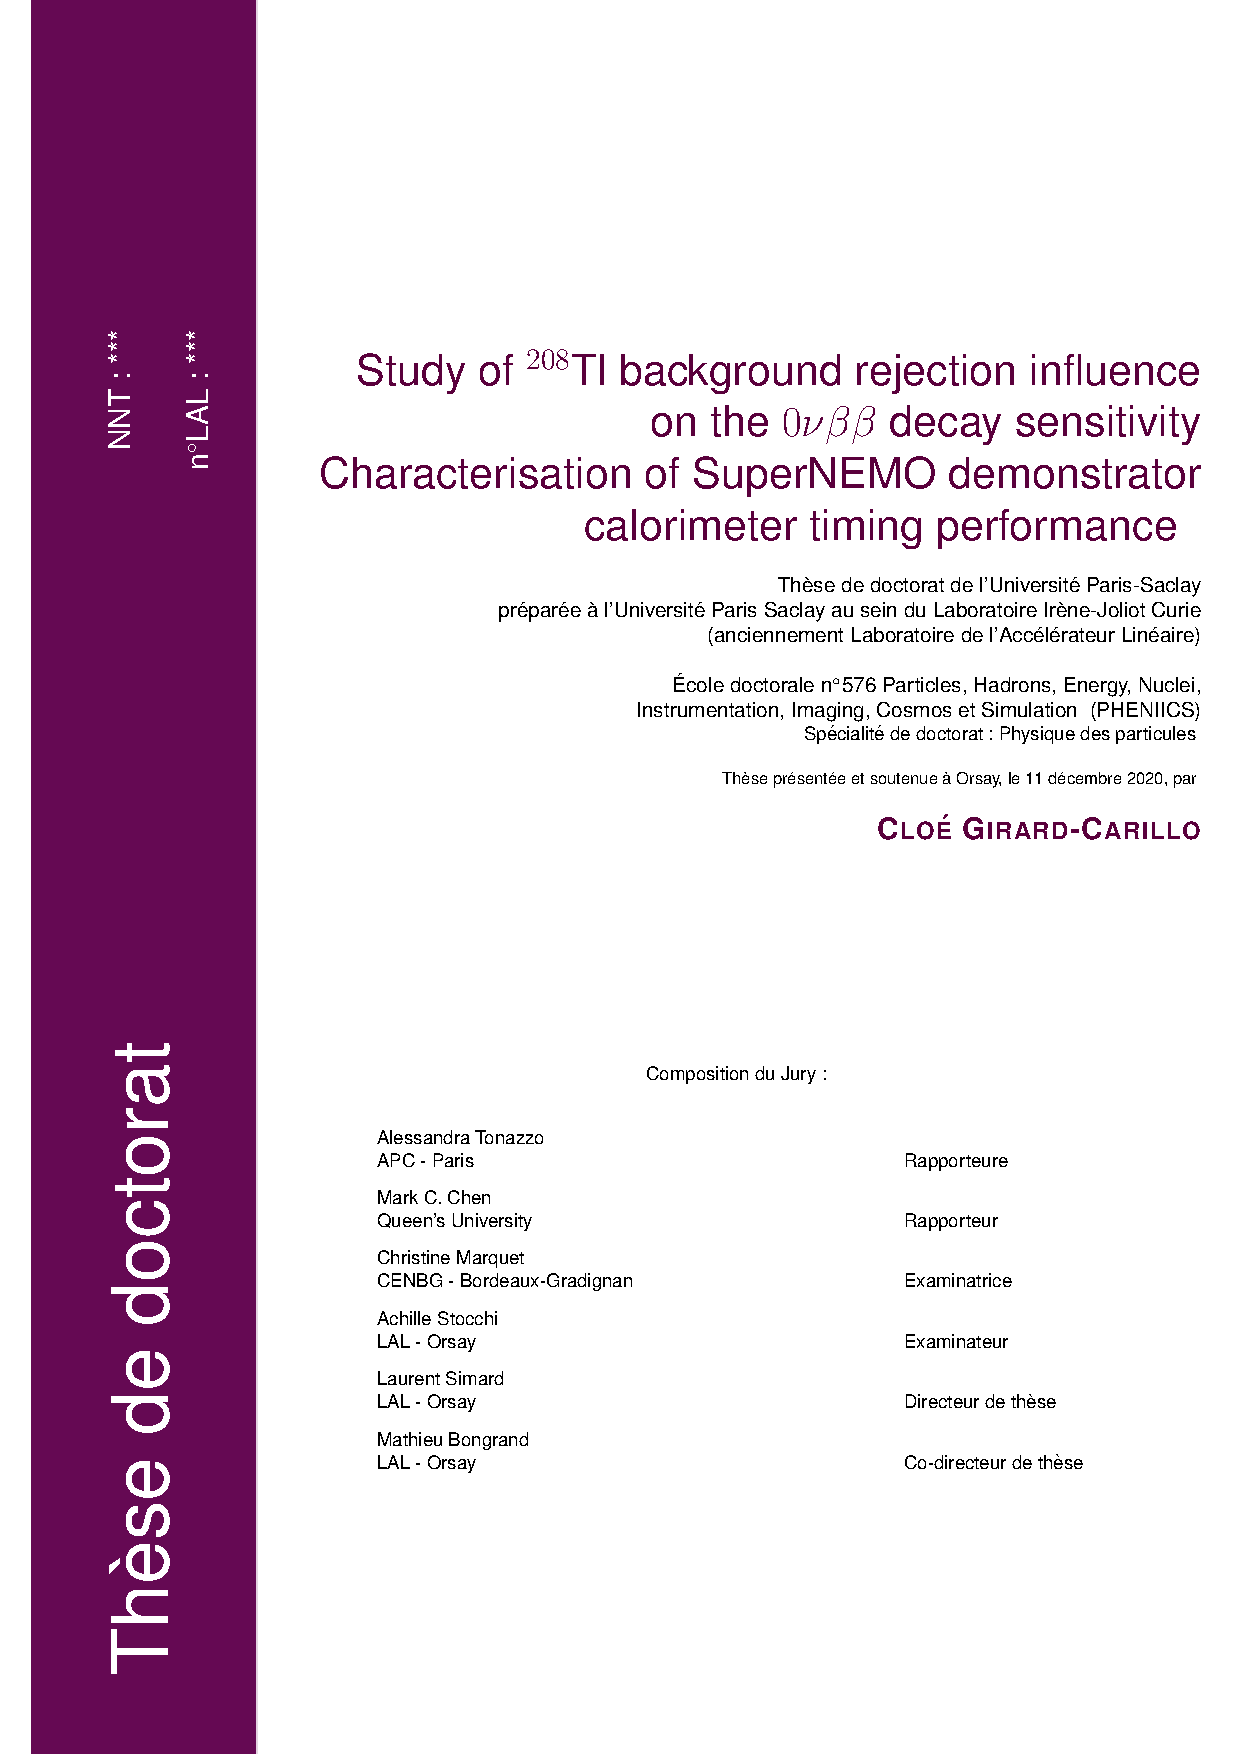
\includepdf{1couverture}
\cleardoublepage
\tableofcontents

\chapter*{Introduction}
\label{ch:intro}
\addcontentsline{toc}{chapter}{Introduction}

It is always interesting to take a historical approach when talking about a scientific discovery. This allows us to put into perspective knowledge that is now considered to have been acquired.

The Standard Model of Elementary Particle Physics attempts to describe the world around us on scales that were inconceivable two centuries ago.
A little over a hundred years ago, Henri Becquerel discovered what we today call radioactivity, with the observation of $\beta$ decay.
This historical discovery was nevertheless accompanied by profound questioning, since the $\beta$ particle emitted during this decay, which turned out to be an electron, only carries away part of the available energy for the reaction.
This observation was contrary to the first principle of thermodynamics on the energy conservation, and some scientists postulated that this fundamental law was being violated.
It took 35 years for an eminent scientist by the name of Wolfgang Pauli to propose as a ``desperate remedy'' the existence of the \emph{neutrino} ($\nu$) - for small neutron in Italian - to explain the problem of missing energy.
Three years later Enrico Fermi laid the foundations for the first mathematical formulation of what is today the Lagrangian of weak interaction.
It was another 25 years, 60 years after the discovery of $\beta$ radioactivity, before the neutrino was experimentally observed by Clyde Cowan and Frederick Reines.
The neutrino adventure had only just begun.

Why is this particle, although abundantly produced in the sun in the atmosphere and in the earth, so difficult to detect?
It is because of its very low interacting rate with the matter - electrons and quarks - that constitutes us, being sensitive only to the weak interaction (of short range), and to the gravitational force (very weakly since the mass of the neutrino is extremely low, so much that it was believed massless for a long time).

In the current model of particle physics, neutrinos are actually described as massless.
It was Bruno Pontecorvo who proposed in 1957 that neutrinos could oscillate between their different mass states, based on the already known model of oscillation of neutral kaons.
To be valid, this model then presupposed that neutrinos had a non-zero mass.
It was the SuperKamiokande experiment that first observed this phenomenon in 1998, demonstrating that at least two of the three neutrino mass eigenstates have a non-zero mass.
The Standard Model of particle physics is then no longer sufficient to account for this particle properties, opening the way to physics beyond the Standard Model.

It now remains to be discovered how this particle acquires its mass.
Indeed, having a neutral charge under the three fundamental interactions described by the Standard Model, two mass generation mechanisms are foreseeable.
The first is to assume that, like all other fermions, the neutrino obtains its mass through the Higgs mechanism, leading irremediably to the assumption of the existence of a sterile neutrino.
The second, proposed by Ettore Majorana, assumes that the neutrino is its own antiparticle, giving the neutrino its mass with the addition in the Lagrangian of the Majorana mass term.
If this assertion is the one that applies to neutrinos, then a disintegration, prohibited in the Standard Model, is possible.
It is called \emph{neutrinoless double beta decay} ($\zeronu$), to contrast with the \emph{two neutrinos double beta decay} ($\twonu$) allowed by the Standard Model and already observed for several isotopes.
In the former disintegration, two simple $\beta$ decays take place simultaneously in the same nucleus, in which the two neutrinos are absorbed, allowing the total energy of the reaction to be distributed between the two exiting electrons.
For reasons that are detailed in the first chapter of this manuscript, which deals with the phenomenology of the neutrino, this disintegration is only possible if the neutrino is a Majorana particle.

Several experiments, also described in the first chapter, are dedicated to the search for this disintegration which, if it exists, is expected to be extremely rare.
%%Its observation would prove the neutrino is a Majorana particle.
The SuperNEMO experiment, on which I conducted my PhD, is one of them.
Successor of the NEMO experiments, it uses a unique combination of technologies, described in detail in the second chapter, allowing to trace the path of the electrons resulting from double $\beta$ disintegrations -with a wire chamber-, and also to measure their energies - with a segmented electromagnetic calorimeter.

These experiments differ from one another in the technology they use, and also in the sensitivity they can achieve in the search for this decay.
Within the framework of this PhD, I carried out a sensitivity study of this experiment presented in the third chapter, determining the influence that several characteristics of the detector can have on it.

All these experiments are designed to observe, should this process exist, an extremely rare physical event.
They are thus constrained to focus on the background which may disturb the measurement and have a non-negligible impact on their sensitivity to this disintegration.
In this perspective, the fourth chapter presents a new technique to identify the events resulting from one of the main background for this experiment, which is the natural disintegration of an isotope from the thorium 232 decay chain, found in the detector's sources.
To effectively reject this background, I am also studying the impact of the accuracy of the arrival time measurement in the calorimeter on sensitivity.
To complete this analysis based on detector simulations, the fifth chapter gives an overview of the data taken at Modane with the SuperNEMO calorimeter and of the analysis aiming to characterise the time resolution for a large part of the optical modules.

When I joined the LAL team at Orsay (now IJCLab) as a PhD student, SuperNEMO was already largely built in the Modane underground laboratory.
I had the opportunity to actively participate in the completion of its assembly, as well as in the analyses of the first commissioning data described in the last chapter, thus completing the experimental knowledge acquired during this PhD.

\chapter{Phenomenology of particle physics}
\section{The Standard Model of particle physics}
\subsection{Bosons}
\subsection{Fermions}
\subsection{$\twonu$ decay}
\subsection{Where the Standard Model ends}
\section{Going beyond the Standard Model with neutrinos}
\subsection{Neutrino flavors and oscillations}
\subsection{Neutrino masses and nature}
\label{subsec:nu_mass_nature}
\subsection{Other searches beyond the Standard Model with neutrinos}

\chapter{$\zeronu$ experiment status}
\section{Experimental design criteria}

As no neutrinos are emitted in a $\zeronu$ decay, the minimal observable in direct searches for $\zeronu$ decay is the total energy of the two emitted electrons.
Depending on experiment designs and purposes (detailed in Sec.~\ref{sec:zeronuexp}), individual electron energies and tracks also represent interesting observables.
The signature of a $\zeronu$ signal is an excess of events, compared to the expected background noise, in the total energy spectrum, near the $\Qbb$ released energy.
How large is this peak depends on the energy resolution of the detector.
Research for this signal involves optimising a \emph{region of interest} (ROI), also depending on the energy resolution.
The total number of events $N^{0\nu}$ occuring in the ROI and in the measurement time $t$, for a detector with an detection efficiency $\epsilon$, using a source isotope of $W$ atomic molar mass and $a$ isotopic abundance, is defined as
\begin{equation}
  N^{0\nu}=\ln(2)\frac{\mathcal{N}_{A}}{W}\left(\frac{a\epsilon M t}{\Tbeta}\right)\,\text{,}
  \label{eq:Nevents}
\end{equation}
where $\mathcal{N}_{A}$ is the Avogadro number.
If no excess of events is observed, the limit set on the $\zeronu$ decay half-life is
\begin{equation}
  T_{1/2}^{0\nu\text{,lim}}=\ln(2)\frac{\mathcal{N}_{A}}{W}\left(\frac{a\epsilon M t}{N_{\text{exc}}}\right)\,\text{,}
  \label{eq:Tlim}
\end{equation}
$N_{\text{exc}}$ being the number of $\zeronu$ events excluded at a given confidence level in the ROI.
Then, this sensitivity to the $\zeronu$ decay would depend on the number of total counts in the ROI, some of them possibly being background events:
\begin{equation}
  T_{1/2}^{0\nu\text{,lim}} \propto \left\{
  \begin{array}{ll}
    a M \epsilon t & \text{if no background is expected,} \\
    a \epsilon \sqrt{\frac{M t}{B \Delta E}} & \text{with background.}
  \end{array}
  \right.
  \label{eq:sensitivity_background}
\end{equation}
Here $B$ is the background rate usually expressed in $\Bckunit$ (when normalised to the width of the ROI, the source mass, and the observation time) and $\Delta E$ is the energy resolution.
The advantage of a background free experiment clearly comes out: the $\zeronu$ half life would increase linearly with the time of exposure $t$ (as opposed to $\sqrt t$ for an experiment with a large number of background events).
Then, it is clear that the control and the discrimination of background is of high priority for such $\zeronu$ direct search experiments.
We will discuss in Chap.~\ref{ch:detector} some important point to reduce the backgrounds for the $\zeronu$ decay detection.
Next to that, the previous expression fixes the choices that experimenters can make in designing a detector.
An ideal isotope would have a high natural abundance and would be deployed with the higest mass possible in a detector with a high detection efficiency, a good energy resolution (small $\Delta E$) under low-background conditions (small $B$).
Of all the $35$ isotopes capable of disintegrating through $\twonu$, none meets all the previous conditions.
Expermimenters will then have to find compromises, which are at the origin of the different detection strategies.
Detector can ether use an active or passive source.
In the first case, the source is also the detection medium (detector technologies detailed in Sec.~\ref{subsec:semiconductors},~\ref{subsec:bolometers} and~\ref{subsec:scintillators}).
In the second case, the source is decoupled from the detection part of the experiment (see Sec.~\ref{subsec:TPC} and~\ref{subsec:trackocalo}).
In the next section, we provide a review of the current and future experiments that aim to discover the neutrinoless double beta decay.

\subsection{Aspects of the nuclear matrix elements}
\label{subsec:matrix_element}
\subsection{Quenching}
\label{subsec:quenching}

\section{$\zeronu$ direct search experiments}
\label{sec:zeronuexp}
\subsection{Semiconductors}
\label{subsec:semiconductors}
Various semiconductor technologies are employed in the detection of $\zeronu$ decay.
The $^{76}$Ge $\beta\beta$ emitter ($\Qbb=2039$ keV) is historically important as it has been adopted since the 1960s in $\zeronu$ decay searches, acting as active source, which enhances the detection efficiency.
$^{76}$Ge-enriched high purity Germanium detectors (HPGe) offer both high energy resolution and extremely high radiopurity (as impurities are removed in the crystal growing process).
These characteristics allow, once external background contribution is minimised, to reach high sensitivity on $\zeronu$ decay, which makes this category of detectors one of the most promising for ton-scale experiments.
Since the last generation (IGEX and Heidelberg-Moscow), HPGe detectors had been improved to reach an ultra low background rate, making way for the current generation of $\zeronu$ detectors -- GERDA, MAJORANA demonstrator and LEGEND.\\

The \textbf{GERDA} experiment (GERmanium Detector Array) is located at the Laboratori Nazionali del Gran Sasso (LNGS), Italy.
GERDA phase I was running from $2011$ to $2013$ with $17.8$ kg of enriched active source detectors from the HEIDELBERG-MOSCOW and IGEX experiments.
Its first aim was to put to the test the controversial result of HEIDELBERG-MOSCOW experiment given in $2001$, announcing the first evidence for $\zeronu$ signal at a $4.2\sigma$ confidence level.
With an exposure of $21.6$ kg.y, the absence of signal in the GERDA-I experiment refuted the previous result, setting a limit $\Tbeta>2.1\, 10^{25}$ y.
Since $2015$, the GERDA experiment is in the second phase (see Fig.~\ref{fig:GERDA}), with a total of $35.8$ kg enriched detectors, $20$ kg of which is Broad Energy Germanium (BEGe) detectors that have been deployed for GERDA-II, providing a better energy resolution and pulse shape discrimination.
The active source is deployed inside a liquid Argon (LAr) augmented with light sensors, acting as an active external shield as well as a cooling down system.
The total is surrounded by a water tank.
The aim is to reach a $10^{26}$ y sensitivity with $100$ kg.y exposure, and a background rate less than $10^{-3}$ $\Bckunit$.
The underground laboratory of INFN provides $3500$ m water equivalent to reduce the external cosmic background.
In $2019$, a combined analysis for GERDA phases I and II has resulted in a half-life limit of $\Tbeta>0.9\, 10^{26}$ y ($90$\% C.L., sensitivity assuming no signal is $1.1\, 10^{26}$), corresponding to an effective neutrino mass of $\mbb<0.07\text{-}0.16$ eV ($90$\% C.L.)\footnote{This result depends on the nuclear matrix elements used for the calculations. See Sec.~\ref{subsec:matrix_element}.}.


\begin{center}
  \begin{table}
    \begin{tabular}{l  c  c  c  c}
      \hline \hline
      Experiment &  Isotope  & M (kmol)&$\Tbeta$ ($90$ \% C.L.)&  $\mbb$ (meV)\\
      \hline
      GERDA~\cite{art:GERDA2019}        & $^{76}Ge$  & $0.41$  & $9\,10^{25}$          & $104-228$    \\
      MAJORANA~\cite{art:majorana2019}  & $^{76}$Ge  & $0.34$  & $2.7\,10^{25}$        & $157-346$    \\
      CUPID-$0$~\cite{art:CUPID2018}    & $^{82}$Se  & $0.063$ & $0.24\,10^{25}$       & $394-810$    \\
      CUORE~\cite{art:CUORE2018}        & $^{130}$Te & $1.59$  & $1.5\,10^{25}$        & $162-757$    \\
      EXO-$200$~\cite{art:EXO2018}      & $^{136}$Xe & $1.04$  & $1.8\,10^{25}$        & $93-287$     \\
      KamLAND-Zen~\cite{art:KamLAND2016}& $^{136}$Xe & $2.52$  & $10.7\,10^{25}$       & $76-234$     \\
      \hline \hline
    \end{tabular}
  \end{table}
\end{center}


\begin{figure}
  \centering
  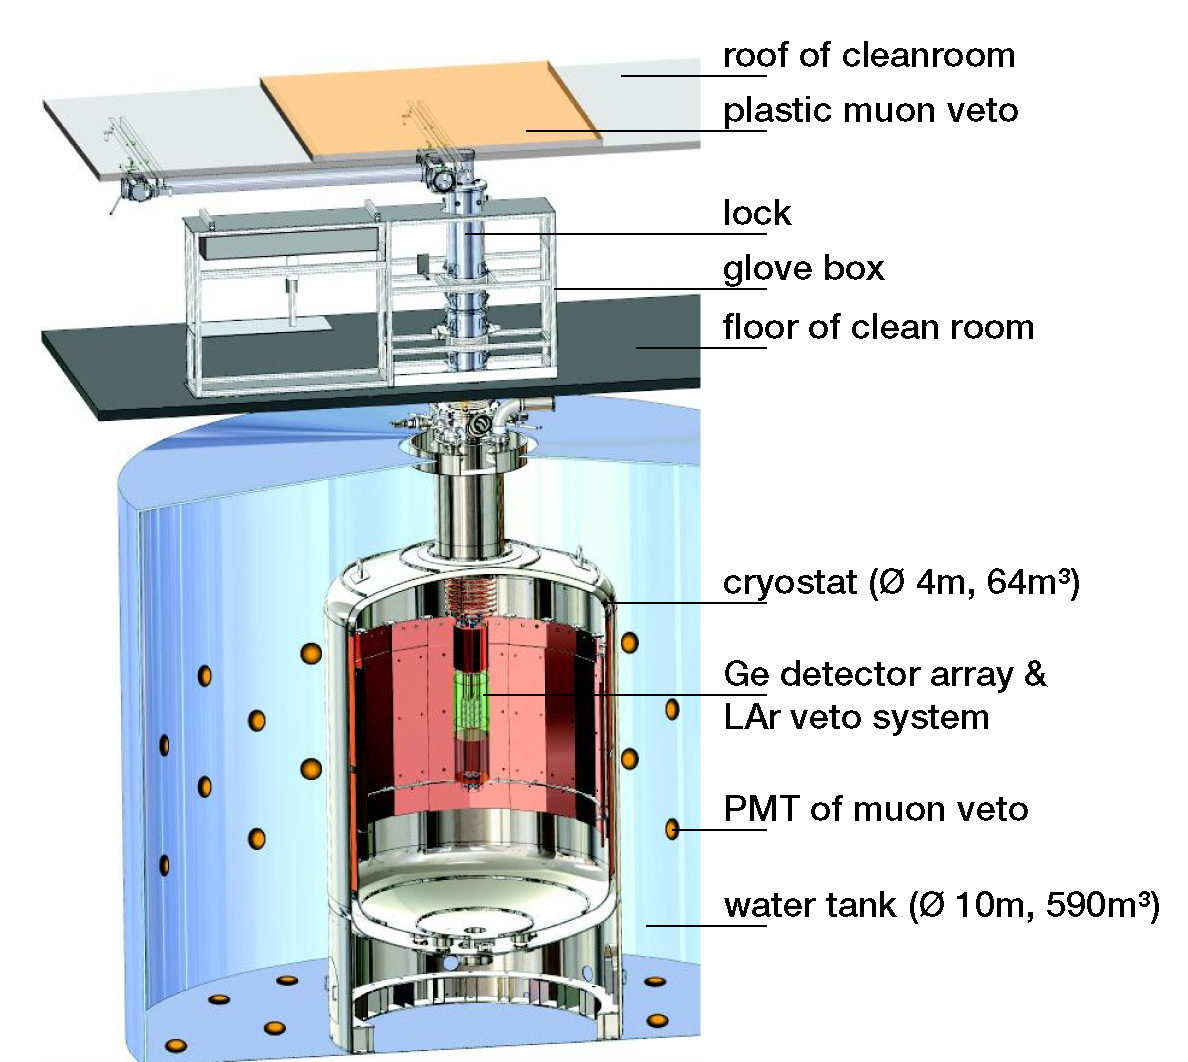
\includegraphics[width=10cm]{0nubbexperiments/fig_0nubbexperiments/GERDA.png}
  \caption{\label{fig:GERDA}}

\end{figure}


\textbf{MAJORANA demonstrator}

\textbf{LEGEND}
\subsection{Bolometers}
\label{subsec:bolometers}

Bolometers are high energy resolution and high detection efficiency calorimeters operating at low temperatures ($\simeq 10-20$ mK).
This type of detector is particularly suitable for $\zeronu$ searches, with the possibility of building large-scale experiments.

\textbf{CUORE}\\
\textbf{CUPID}\\
\textbf{AMoRE}
\subsection{Time projection chambers}
\label{subsec:TPC}

Time Projection Chambers (TPC) detectors use a medium producing two ways to measure the electron energies: a \emph{scintillation} (ultra-violet light) prompt signal, and a \emph{ionisation} delayed signal.
When a particle crosses the detector, a scintillation light is emitted, the energy of the scintillation peak depending on the medium.
Scintillation photons, travelling at speed of light in the medium, are detected by photosensors, giving the \emph{zero-time} of the event.
The crossing particle ionises the medium all along its way, creating electrons drifting to a collection system (an electric field is applied between cathode and anode), allowing the precise measurement of the electron production location in a 2D plane.
The drift time measurement gives access to the third coordinate of the interaction point.
Therefore, combining the two consecutive signals allows precise position and energy reconstruction.
An discriminating observable is the ionisation-to-scintillation ratio (see Fig.~\ref{fig:ratio_EXO-200}) as it provides particle discrimination between $\alpha$ particles (low ratio) and $\gamma$ radiations and $\beta$ particles (high ratio).
For $\zeronu$ searches, $^{136}$Xe-enriched isotope in liquid phase is used, offering a maximal source density (more compact detecors) and a good position resolution.
Unfortunately, the energy resolution is worse than that of the gas-phase TPCs detectors\footnote{Two-phase liquid-Xenon detectors are developed for Dark Matter searches and could be exploited for $\zeronu$ direct searches with the DARWIN project.}.
Noble elements are natural radiation detectors, avoiding the need for excess materials that could generate extra radioactive backgrounds.
$^{136}$Xe-enriched is the only noble element capable to $\twonu$ decay, with $\Qbb=2457.8$ keV.
This isotope has a relatively high natural abundance ($9$\%), can be enriched to highly pure concentrations, and does not have other long-lived radioactive isotopes, making it interesting for large-scale TPCs $\zeronu$ experiments.\\

The \textbf{EXO-$200$} experiment is a prototype of the Enriched Xenon Observatory (EXO) project, currently operating in a room under an overburden of $1624$ m.w.e, at the Waste Isolation Pilot Plant (WIPP), USA.
The detector is shaped as a cylinder, with two back-to-back cylindrical TPCs.
A high negative voltage grid cathode helds at the mid plane of the detector ($40$ cm diameter), and two anodes are located on both sides, at ground potential.
A cross-section of the detector is displayed in Fig.~\ref{fig:EXO-200}.
With $110$ kg of enriched $^{136}$Xe in liquid phase (the detector is held at $167$ K in a cryongenic bath), the phase I of this TPC detector has measured for the first time the Xenon $\twonu$ decay with $\Tbeta=2.165\times 10^{21}$ y.
Between phase I and IIa, the detector was upgraded with improved low-noise electronics, a Radon suppression system, and the impurities contents of the Xenon were reduced by a factor ten.
The current detector performance shows an energy resolution of $2.90$\% (FWHM) at the decay $Q$-value and a background rate of $(1.6)\times 10^{-3}\Bckunit$.
EXO-$200$ phase IIa data placed a new limit of $\Tbeta>1.8\times 10^{25}$ y ($90$\% C.L.).
The final analysis of data is in progress.


\begin{figure}
  \centering
  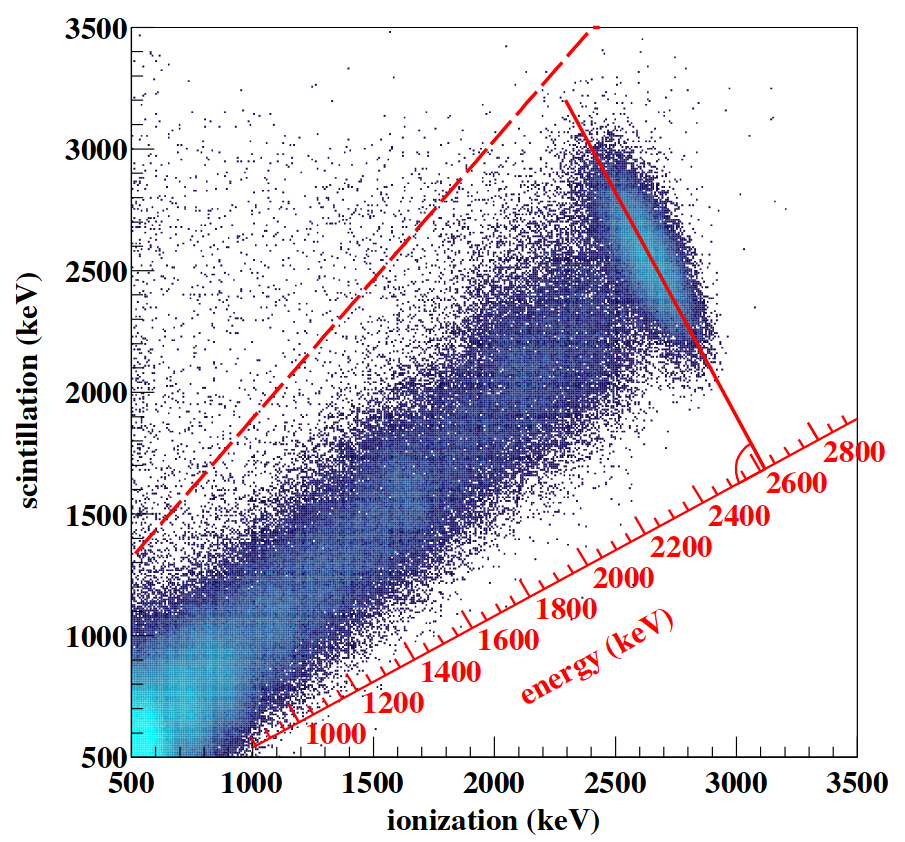
\includegraphics[width=8cm]{0nubbexperiments/fig_0nubbexperiments/ionisation-to-scintillation_EXO-200.png}
  \caption{\label{fig:ratio_EXO-200}}

\end{figure}

\begin{figure}
  \centering
  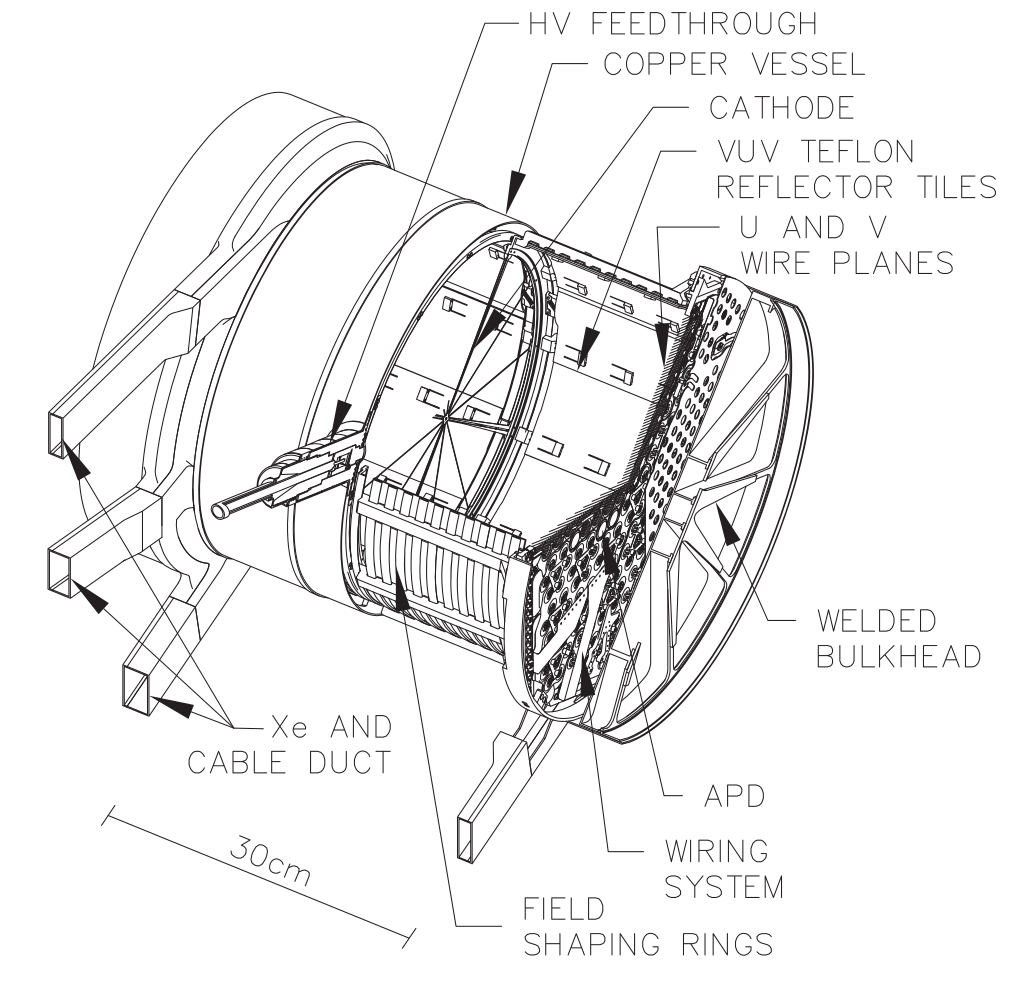
\includegraphics[width=8cm]{0nubbexperiments/fig_0nubbexperiments/EXO-200.png}
  \caption{\label{fig:EXO-200}}

\end{figure}

\textbf{nEXO}\\
\textbf{NEXT}\\
\textbf{PandaX-III}
\subsection{Scintillators}
\label{subsec:scintillators}
\textbf{KamLAND-ZEN and KamLAND2-ZEN}\\
\textbf{ZICOS}\\
\textbf{CANDLES}
\subsection{Tracking calorimeters}
\label{subsec:trackocalo}
Tracking calorimeters technology, instead of using a \emph{source-as-detector}, employ a passive source shaped as thin source foils of enriched $\beta\beta$ emitters.
Sources are placed at the detector centre, surrounded by two trackers allowing for particle identification (between electrons, positrons, $\gamma$ and $\alpha$ particles) and vertex reconstruction to improve the background rejection.
The whole is sandwiched between calorimeters enabling individual particle energy reconstruction.
In case of a discovery, this passive source tracking calorimeter technology provides topological information on angular emissions of the two electrons from $\beta\beta$ decay, making possible to distinguish between underlying mechanisms for $\zeronu$ decay (see Sec.~\ref{subsec:nu_mass_nature}).\\

The \textbf{SuperNEMO} experiment is a next-generation of detector, inheriting the lineage of the NEMO (Neutrino Ettore Majorana Observatory) experiments, which successfully studied multiple isotopes as enriched Molybdenum $^{100}$Mo.

\chapter{The SuperNemo demonstrator}
\label{ch:detector}

\section{The SuperNemo demonstrator}
\subsection{Comparison with Nemo$3$ experiment}
\subsection{Expermimental design}
\subsection{Sources}
\subsection{Tracker}
\subsection{Calorimeter}
\label{subsec:SN_calo}



\subsubsection{Scintillator}





\subsubsection{Photomultiplier}
\label{sec:calorimeter}
\subsection{Calibration systems}
\subsection{Control Monitoring system}
\subsection{Electronics}

\section{The backgroung of SuperNEMO}
\label{sec:SNbkg}
\subsection{Internal background}
\label{subsec:SNbkg_internal}

Trace quantities of naturally-occurring radioactive isotopes can occasionally produce two-electron events and thus can mimic $\beta\beta$-decay events.
The largest contributions come from isotopes of decay chains of $^{238}$U, $^{232}$Th and $^{40}$K, which disintegration occur inside the source foils, as well as inside the tracking volume.

Décire la contamination mesurée des sources, et du radon dans la partie suivante

\subsection{External background}
Radon:\\
Radon is a noble gas which occurs as an indirect decay product of uranium and thorium.
Due to its chemical properties, radon has a long diffusion length in solids, making it difficult to remove.
Radon contaminations inside the tracker volume is a major background to the rare event experiments such as SuperNEMO.
Simulations show that, to achieve the designed sensitivity, the level of radon must not exceed $0.15$ mBq/m$^{3}$ since its decay daughter \Bi, $\Qbb= 3.2$ MeV can mimic a $\zeronu$ event.
Radon concentration measurements inside the demonstrator tracker have been performed by the SuperNEMO collaboration, revealing an activity of $0.15\pm0.02$ mBq/m$^{3}$, through the combination of an anti-radon tent and an air-flushing method.

%%Repris d'un article -> a changer:
They are outgased in the air from the rock walls of the experimental hall and can enter the detector either through tiny gaps between sectors or through gas pipe joints.
The progeny of radon and thoron produces $\gamma$-rays and $\beta$ decays accompanied by internal conversion (IC), Møller or Compton scattering.
\subsection{Background specifications}
\subsection{Measured demonstrator background levels}

\section{Magnetic field}
\label{sec:magnetic_field}

It is, however, not high enough to impact significantly neither the few muons nor the $\alpha$ particles expected to be detected by the tracker.
Due to their much higher momenta, they will instead leave straight tracks in the wire chamber.

\section{The SuperNemo software}
\label{sec:SNsoftware}
\subsection{Simulation}

As described in Sec.~\ref{sec:SNsoftware} of Chapter~\ref{ch:detector}, the SuperNEMO collaboration developed its own simulation, reconstruction and analysis environment.
The Falaise software, specifically designed by and for the SuperNEMO collaboration, holds the \verb!C++! library for the event reconstruction and analysis of simulated and real data.
Especially, it contains the geometry, the detector material, the event data model, the reconstruction algorithms and the data analysis.
Finally, the SNFee software is a tool package for the configuration, control and monitoring of the SuperNEMO front-end electronics.

\subsection{Reconstruction}

\chapter{Analysis tools}

\section{Internal and external probabilities}
\subsection{Internal probability}
\label{subsec:internal_prob}
Internal probability is a mathematical tool used to quantify the probability that two particles (in this study only electrons will be considered) were emitted simultaneously and at the same location in the source foils.
The internal probability is defined from the associated internal $\chi^{2}$
\begin{equation}
  \chi^{2}_{int}=\frac{((t^{exp}_{1} - \frac{L_{1}}{\beta_{1} c}) - (t^{exp}_{2} - \frac{L_{2}}{\beta_{2} c}))^{2}}{\sigma_{tot}^{2}}\,\text{,}
  \label{eq:int_chi2}
\end{equation}
where c is the speed of light, $t^{exp}_{i}$ is the time measured in calorimeters for the particle $i$, $L_{i}$ is the reconstructed track length, and $\beta_{i}$ is defined as $\sqrt{E_{i}(E_{i} + 2m_{e})} / (E_{i} + m_{e})$, $E_{i}$ being the energy of particle $i$ and $m_{e}$ the electron mass.\\
The denominator in eq.~\ref{eq:int_chi2} is the total uncertainty defined as
\begin{equation}
  \sigma_{tot}=\sqrt{\sigma_{t}^{2}+\sigma_{\left(\frac{L}{\beta c}\right)}^{2}+\sigma_{l}^{2}}\,\text{,}
  \label{eq:sigma_tot}
\end{equation}
where the first term $\sigma^{2}_{t}=\sum_{i=1,2}\sigma^{2}_{t_{i}}$ is the uncertainty the time measurement in the calorimeters with $\sigma_{t}$ defined as
\begin{equation}
  \sigma_{t}=\sqrt{\dfrac{\tau_{\text{SC}}^{2}+\left(\dfrac{\text{FWHM}(\text{TTS})}{2\sqrt{2\ln{2}}}\right)^{2}}{\text{N}_\text{PE}}}\,\text{.}
  \label{eq:sigma_t}
\end{equation}
The second term $\sigma^{2}_{\left(\frac{L}{\beta c}\right)}=\sum_{i=1,2}\sigma^{2}_{\left(\frac{L_{i}}{\beta_{i}c}\right)}$ is the uncertainty depending on the energy of electron $i$ as
\begin{equation}
\sigma_{\left(\frac{L}{\beta c}\right)} = \biggl\lvert \dfrac{\partial t_{th}}{\partial E}  \biggr\rvert \Delta E\,\text{.}
  \label{eq:sigma_L}
\end{equation}
The third term $\sigma_{L}$ represents the typical uncertainty due to track reconstructions of particles\footnote{This value is set to $\sigma_{L}=0.03$ ns in a first approximation (see chapter -ref-).}.\\
Then the internal probability evaluate the difference between experimentally measured time and theoretical times.




\section{Simulations}
\subsection{Modifications of simulation software}
\subsection{Internal background simulations}
\subsection{$\zeronu$ simulations}

\chapter{Improvement of the rejection of the internal Thallium-$208$ background}
\label{ch:timediff}

At the end of September 2018, the Selenium-$82$ source foils were installed on the demonstrator.
At this time, the internal \Tl\ and \Bi\ activities had already been measured by the BiPo detector.
In this chapter, we focus on rejection techniques optimised to have a high efficiency on internal \Tl\ events.



\section{Motivations for this study}

We discussed in chapter~\ref{ch:sensitivity} about the specified levels of contamination inside the source foils.
These levels are embeded by the internal \Bi\ and \Tl\ activities, given in Tab.~\ref{tab:real_target_act}.
These specifications aimed at reaching the targeted \Se\ half-life limit of $\sim1\times10^{26}$~year for a $500$ kg/y exposure.
In the same table are also given the activities measured by the BiPo detector, after the sources production.
These measurements reveal a \Tl\ contamination, about $30$ times higher than expected.
As concluded in the previous chapter, this contamination impacts the sensitivity on the $\zeronu$ decay of the final detector, decreasing it.

In this section, we work to describe the specificities of Thallium-$208$ internal background.
We will see what the methods of rejecting this background already exist.
We will also detail the basic principle of a new method we have put in place, to meet the needs of rejections of Thallium, following the measurements of BiPo.

\subsection{The internal \Tl\ background}

Trace quantities of naturally-occurring radioactive isotopes inside the source foils can occasionally produce two-electron events, and thus can mimic $\beta\beta$-decay events.
The \Tl, a progeny of \U, is one of the largest contribution to the internal background.
In fact, two electrons can be produced via $\beta$-decay followed by a M\o{}ller scattering, $\beta$-decay to an excited state with the subsequent internal conversion, or due to Compton scattering of the de-excitation photon (Fig.~\ref{fig:internal_contamination}).
\begin{figure}
  \centering
  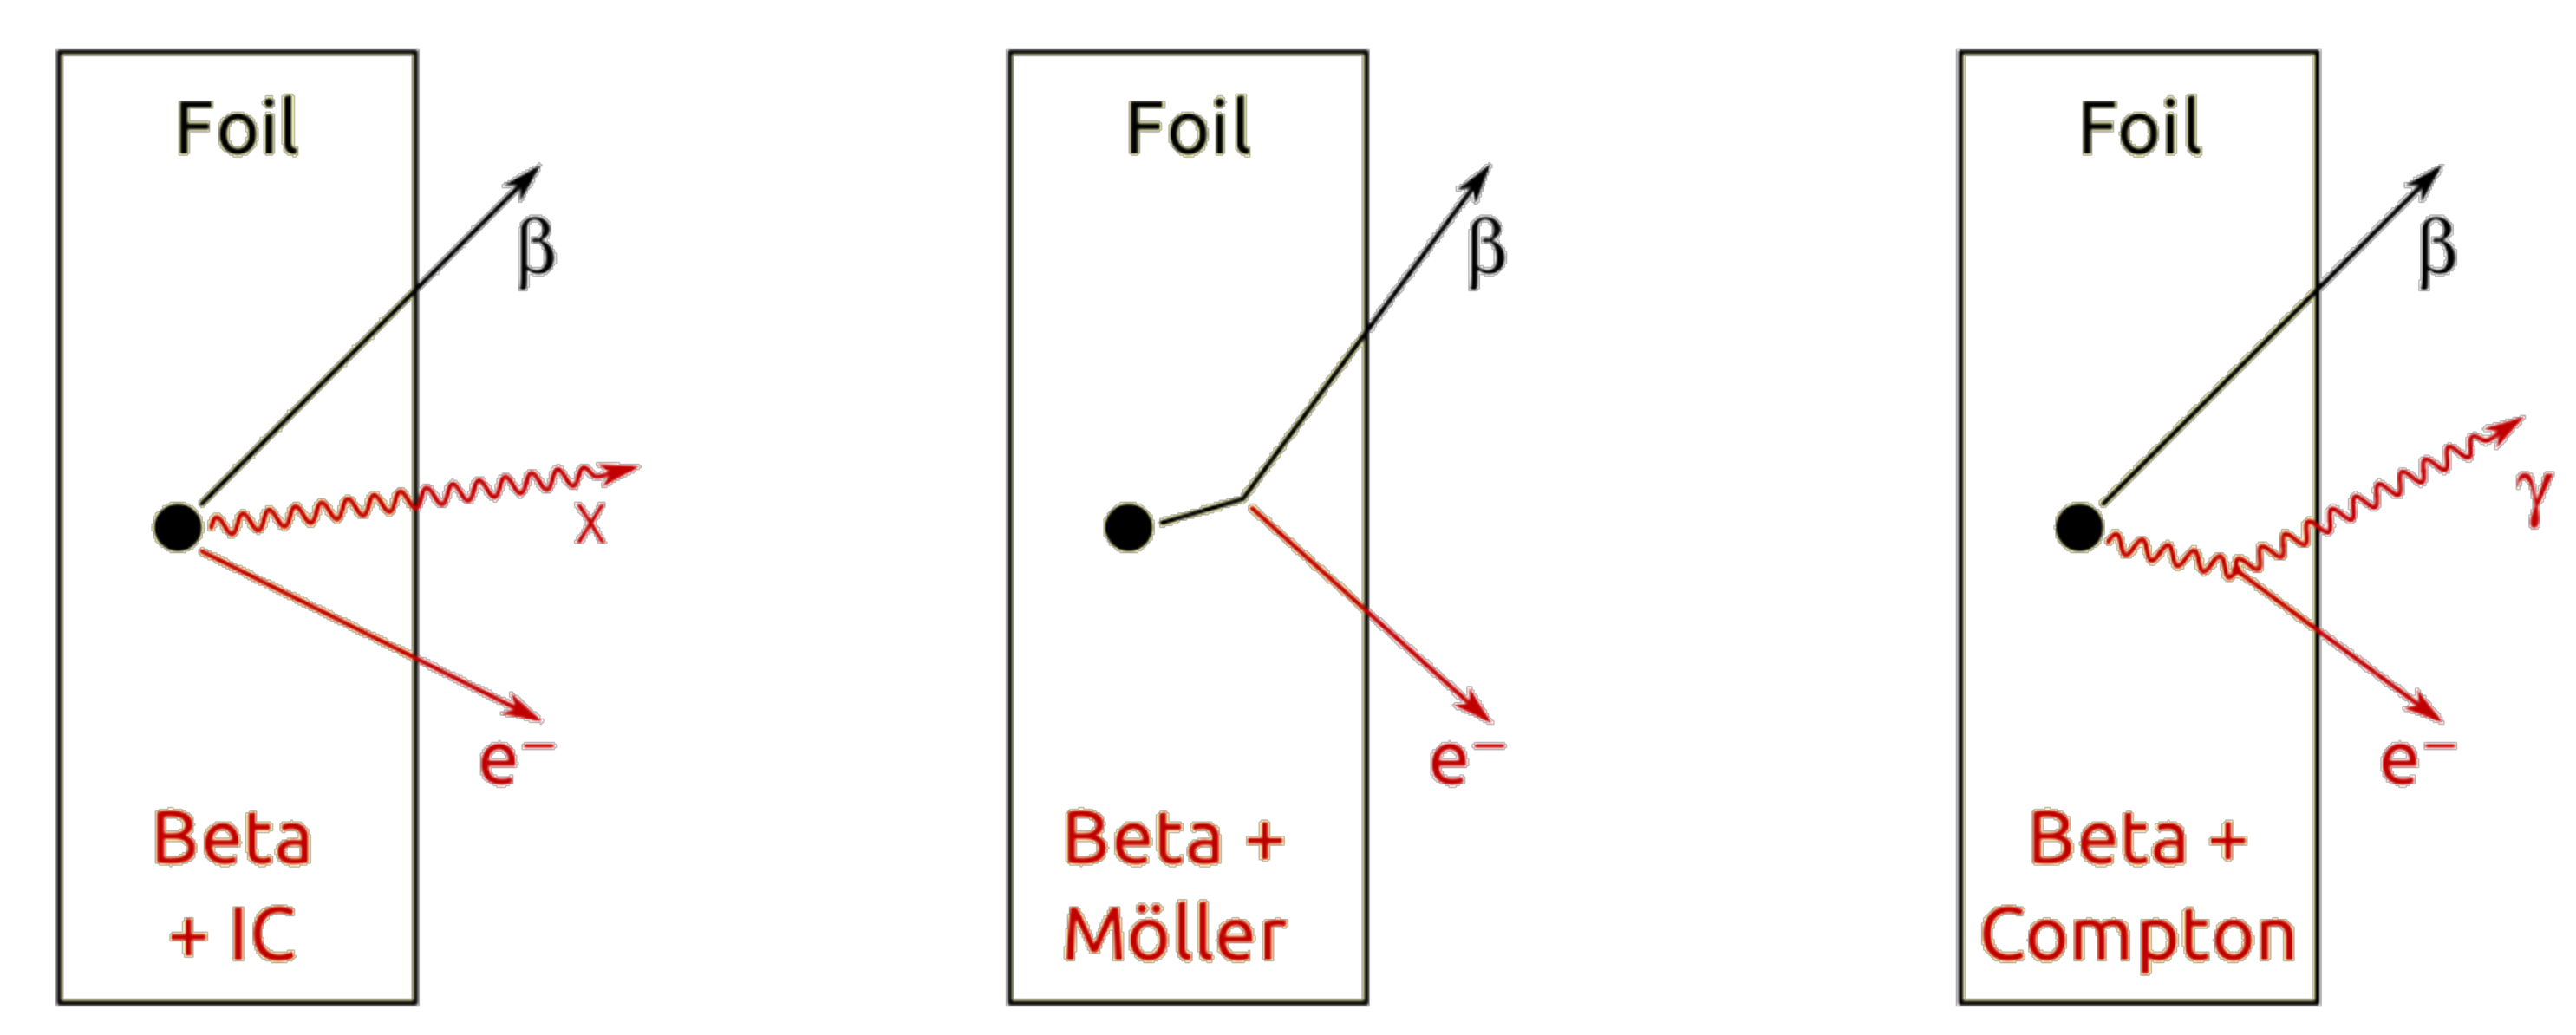
\includegraphics[width=10cm]{timedifference/fig_timediff/internal_contamination.pdf}
  \caption{(a) $\beta$ decay + internal convertion: \Tl\ nucleus performs a $\beta$ decay, then an electron is emitted after internal conversion of photon
    (b) $\beta$ decay + M\o{}ller:
    (c) $\beta$ decay + Compton diffusion: \Tl\ nucleus $\beta$ decays to an exited state, then the photon perfoms a Compton diffusion.
 \label{fig:internal_contamination}}
\end{figure}
%% The ultimate internal background for $\zeronu$ experiments is the $\twonu$ decay of the studied isotope.
%% When present in the source foils, \Tl\ and \Bi\ can mimic the $\zeronu$ signal by different processes (see Fig.~\ref{fig:internal_contamination}).

\subsection{Rejection of the \Tl\ background}
We present a simplified disintegration scheme of \Tl\ in Fig.~\ref{fig:Tl_scheme}.
\begin{figure}
  \centering
  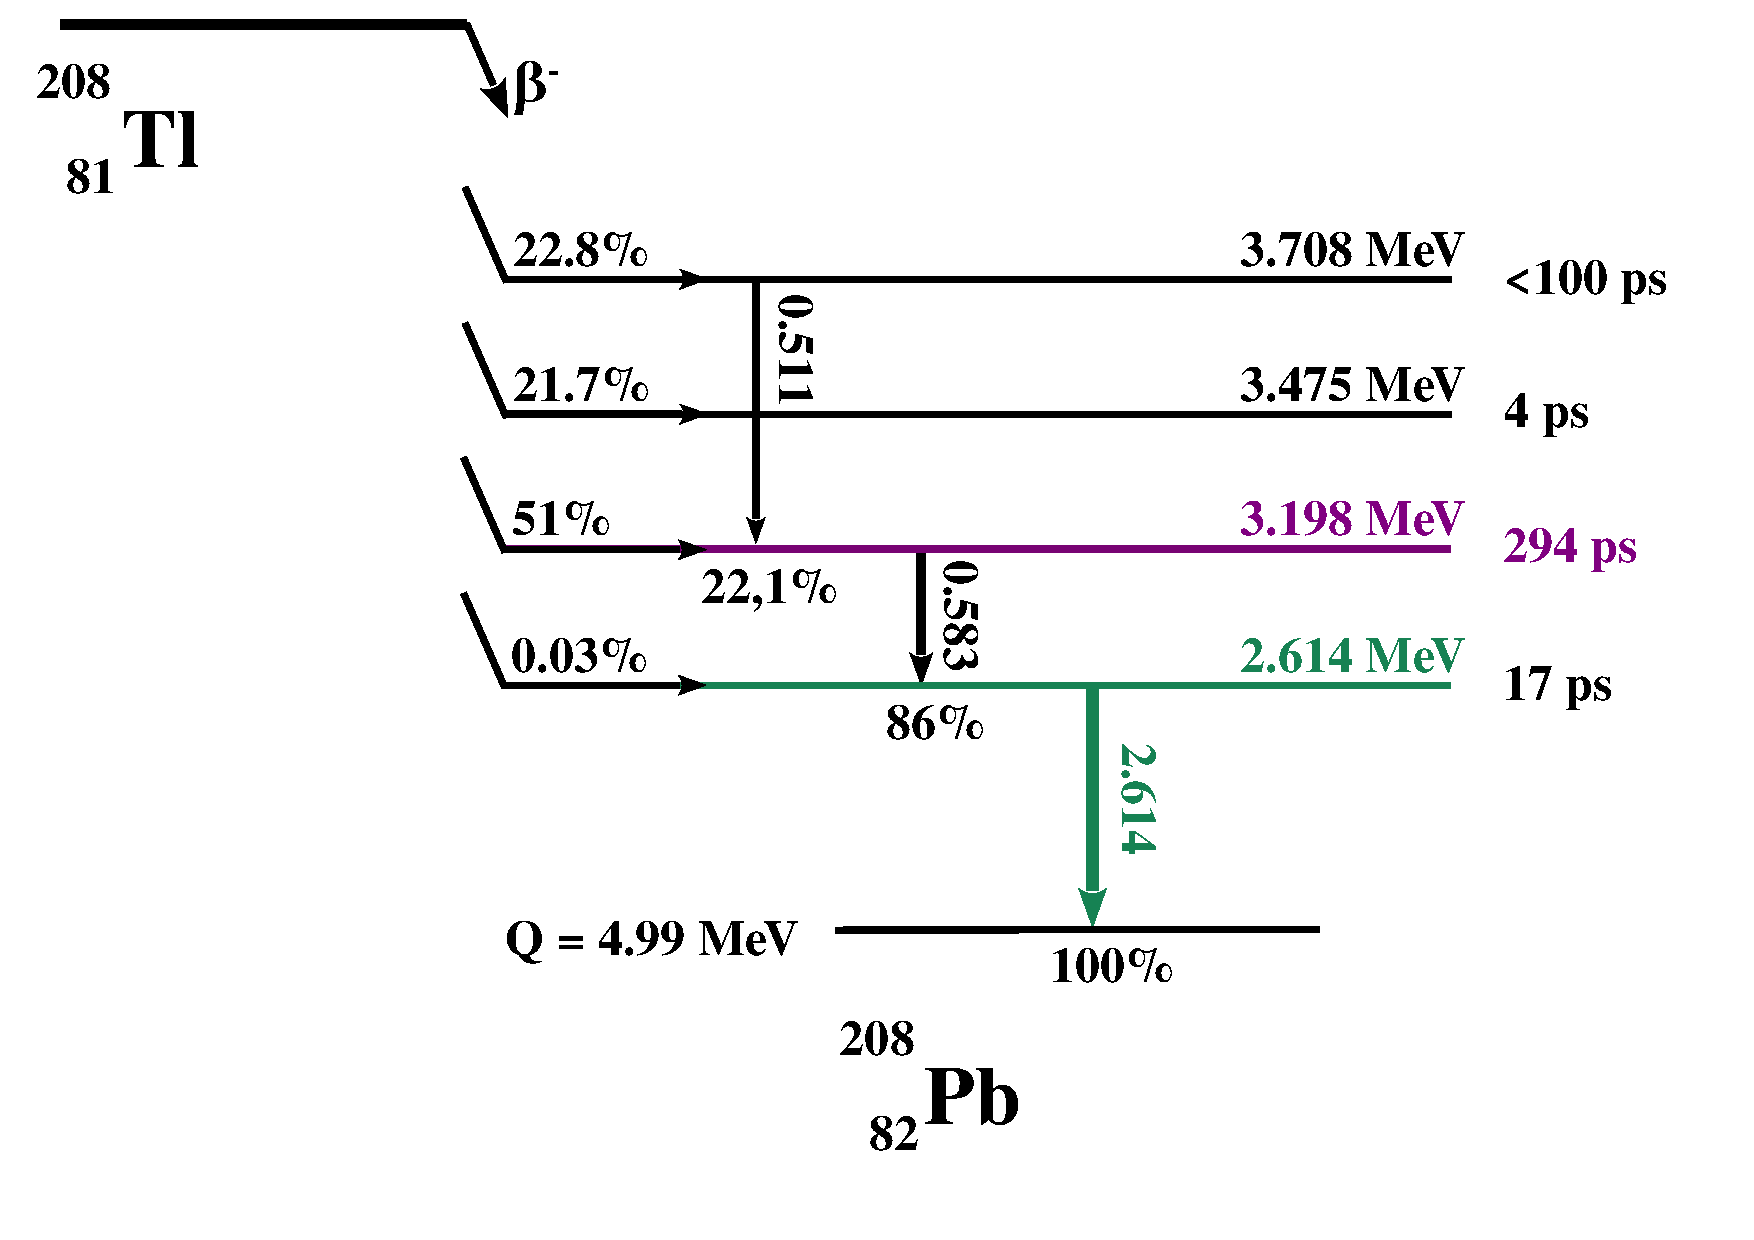
\includegraphics[width=13cm]{timedifference/fig_timediff/Tl_decay_scheme.pdf}
  \caption{Simplified desintegration scheme for \Tl\ isotope.
    The level in red has a significant life time of $294$ ps and can be useful in internal backgroung rejection.
  \label{fig:Tl_scheme}}
\end{figure}


For this study, we are focusing on the internal conversion process coming from the contamination of \Tl\ in the source foils.
Regarding the simplified desintegration scheme of the \Tl\ isotope (Fig.~\ref{fig:Tl_scheme}), we see that the $\beta$ desintegration has $51\%$ of probability to fall on the $294$ ps-life time exited level.
To decay to \Pb, the exited isotope has $100\%$ of probability to decay emmiting a $\gamma$ of $2.6$ keV.
In $0.2\%$ of cases, one of the orbital electron can interact with the exited nucleus and decay through internal conversion.
To summarise, decays where a \Tl\ nucleus emmits a $\beta$ particle and then an electron comming from internal conversion of the $2.6$ MeV-$\gamma$ represents $75\%$ of the total $\beta$ decays.
In this case, the internal conversion electron is time-delayed of $294$ ps compared with the $\beta$ particle.
We aim to use this delayed electron to discriminate \Tl\ internal background from signal and other internal backgrounds.





\begin{itemize}
\item trop de \Tl\ dans les sources par rapport aux spec
\item donc besoin d'une méthode de réjection spécifique pour \Tl\
\item pas gênant au niveau du démonstrateur (pour cela regarde le nombre d'événements de Tl208 attendus après l'optimisation des coupures avec le niveau de Tl208 mesuré par Bipo-3, je pense que c'est moins d'1 evt), mais cela peut être gênant pour une manip à 500 kg.y
\item avant de parler de la réjection avec le temps de vol, parler des autres réjections du Tl208 : bdf interne = 1 électron de conversion + 1 électron bêta -> l'électron de plus haute énergie a un pic en énergie (montrer une figure de simulation pour illustrer) et commenter avec le fait que la résolution en énergie s'améliore entre NEMO-3 et le démonstrateur. Donc normalement cette réjection sur l'énergie individuelle est plus efficace avec le démonstrateur.
\item Schema désintégration
\item Internal conversion -> reconnaître le Tl avec gamma $2.6$ MeV
\item Préciser l'énergie de l'électron de conversion associé (ou plutôt les énergies : raies K, L ...)
\item Un des deux gamma est retardé de 294 ps, puis conversion interne -> donner le proportion (nb d'ev attendus, dans la ROI)
\item Avant d'entrer dans le détail préciser le principe de la réjection par temps de vol.
L'électron de plus haute énergie est en retard, avec un retard en moyenne de 294 ps pour la plupart des niveaux (discuter un peu le schéma de désintégration, dans quel cas il sera en retard).
Ensuite dire que tu as quantifié le pourcentage d'électrons de haute énergie en retard avec une simulation "parfaite" i.e. avec une résolution en  temps  nulle.,
\end{itemize}

%% Internal conversion occurs after $\beta$ or $\alpha$ radioactive decays leaving the nucleus exited.
%% Then a $\gamma$ particle is emitted and transfers its energy to an atomic electron which results in ejection of this electron from the atom.
%% The emitted electron has an energy corresponding to the energy of previously exited nucleus reduced by the electron binding energy.
%% After the internal conversion, electrons reorganise.
%% The hole in internal layer is filled by an electron from an external layer (emitting an X ray).\\
%% The probability for an atomic electron to be ejected decreases with the initial binding energy.
%% Thus, electrons from K layers have a higher probability to be converted (see Fig.~\ref{fig:Tl_IC}).

\section{Describe mathematically internal events}

\subsection{The internal probability}
\begin{itemize}
\item outil déjà existant, déjà utilisé dans NEMO-$3$
\item identifier les ev venant de la source
\item détailler chaque terme
\item étudier l'influence du terme $\sigma_{l}$ dans la proba interne (on avait trouvé 0.03 ns pour avoir une Pint plate pour la 0nu)
\end{itemize}

\subsection{The exponential probability}
\begin{itemize}
\item besoin de décrire les ev conversion interne, avec une loi de probabilité
\item Avec un détecteur qui mesurerait parfaitement les temps et les énergies, la loi t(max) - t(min) serait une loi exponentielle, en pratique il faut la convoluer avec une gaussienne.
\item description de l'exponentially modified gaussian avec les paramètres des deux distrib (expo et gaus)
\item Ici montrer une distribution de Pexp pour des evts Tl208 (si possible aussi uniquement pour les evts Tl208 qui ont un Delta t(resolution parfaite) > 0
\item Decrire aussi comment on passe de la probabilité exponentielle modified gaussian à la probabilité cumulée, qui est celle sur laquelle tu vas couper.
\end{itemize}

\section{Event selection}
\begin{itemize}
\item cut Pint/Pexp
\item Montrer un biplot Pint/Pexp pour les evts Tl208 en représentant la coupure.
\item Optimisation of event selection: cut on delta t
\item 208Tl cut efficiency
\item cut efficiencies on 0nubb and other backgrounds
\item Donner le nb d'ev rejeté sur le nb d'ev total, puis sur le nb d'ev retardés
\end{itemize}

\section{Impact of \Tl\ rejection on the experiment's sensitivity}
Reprendre l'analyse de sensibilité faite avec Axel en rajoutant les cuts Pint/Pexp et delta t pour le final detector

\subsection{Influence of the calorimeter time resolution}
\begin{itemize}
\item Se servir des résultats de $\sigma_{t}$ trouvés au chap.~\ref{chap:Cobalt_study}
\item Mais dire que ces sigmas peuvent être améliorés
\item donc présenter l'évolution des résultats (efficacité de réjection et sensibilité) sur la réjection en fonction de la valeur de sigma t, à faire varier dans un certain range.
\item Tu pourrais avec une figure à 2D où tu montres l'efficacité relative 0nu (égale à 100\% avant cette coupure temporelle) en fonction de la réjection du Tl208 -> cela donne une courbe que tu parcoures et tu cherches à optimiser ton point de fonctionnement.
\end{itemize}


\section{Conclusions}




\begin{figure}
  \centering
  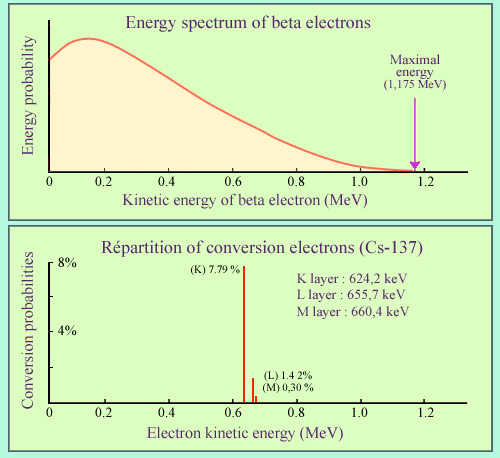
\includegraphics[width=9cm]{timedifference/fig_timediff/SpectreBeta_Cs137.jpg}
  \caption{\label{fig:Tl_IC}}

\end{figure}

\include{efficiency/efficiency}
\chapter{Detector commissioning}
\label{ch:commissioning}

The commissioning of the SuperNEMO demonstrator has begun in $2019$ and first calorimeter data was taken.\\
The calorimeter of SuperNEMO is segmented in $712$ optical modules (OM), each composed by a coupling between a photomultiplier tube (PMT) and a polystyrene scintillator bloc (see Sec.~\ref{subsec:SN_calo} for more details).
The divider of a PMT is connected to $2$ cables, one providing the high voltage (HV), the other one, called signal cable, is a coaxial cable collecting and transporting the charge provided by the PMT.\\
By the summer $2020$, the SuperNEMO demonstrator will be encapsulated in an anti radon tent.
The so called \emph{patch panel} will insure passage of cables from the inside, to the outside of the anti radon tent, therefore doubling the amount of cables needed for the calorimeter.
We refer to the cables running from detector to patch panel as \emph{internal} cables, and the cables from patch panel to the electronic boards as \emph{external} cables.
Consequently, regarding only the calorimeter part, 2848 cables were cut, assembled, connector-mounted, transported and installed at LSM.
Then the check of every cable condition is mandatory to control and eventually fix them.

\section{Reflectometry analysis}
\label{sec:reflecto}

\subsection{Goal of the reflectometry analysis}

Taking into account the final demonstrator design, each coaxial length was determined, cables were cut and labelled in LAL, Orsay.
All external coaxial cables were designed to be $7$ meters-long -- the distance between electronic boards and patch panel being the same for all channels at electronic boards -- and internal cable lengths have been adapted to fit the distance from the patch panel to each optical module.
Then, cutting and labelling all cables lasted several weeks.
After all cables were transported and installed at LSM, we had to check each coaxial cable condition, for several reasons:
\begin{itemize*}
\item check if no cable was damaged during the transport and the installation;
\item control if no swap between cables has been made during cable labelling or calorimeter cabling,
\item check if the coaxial cable was cut at the right length,
\item more importantly estimate the signal time delay due to the cable lengths: knowing that the velocity of electrons in the coaxial cables has a known constant value, the longer is the cable, the more the signal takes time to travel from the PMT to the electronic channel.
  Therefore, each coaxial cable length has to be characterised, especially if we want to do time coincidences between two signals in two different channels.
\end{itemize*}
To do so, a pulse, called \emph{primary} pulse, is generated at the electronic board readout.
The signal will travel all along the coaxial cable, from the electronic board to the PMT divider.
Whether the cable is correctly connected to the PMT or not, the signal reflects at the other end.
\begin{figure}[h]
  \centering
  \begin{subfigure}[b]{0.3\textwidth}
    \centering
    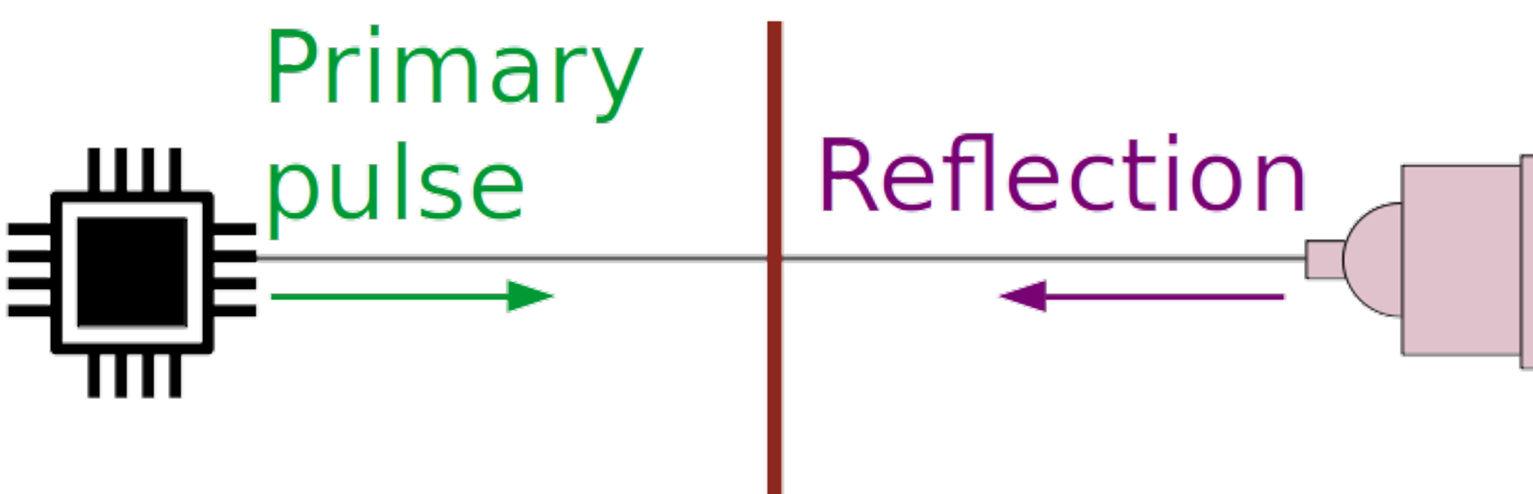
\includegraphics[width=1.1\textwidth]{commissioning/fig_commissioning/scheme_reflecto.pdf}
    \captionsetup{justification=centering}
    \caption{Normal reflection at PMT divider.
      \label{subfig:reflecto_normal}}

  \end{subfigure}
  \hfill
  \begin{subfigure}[b]{0.3\textwidth}
    \centering
    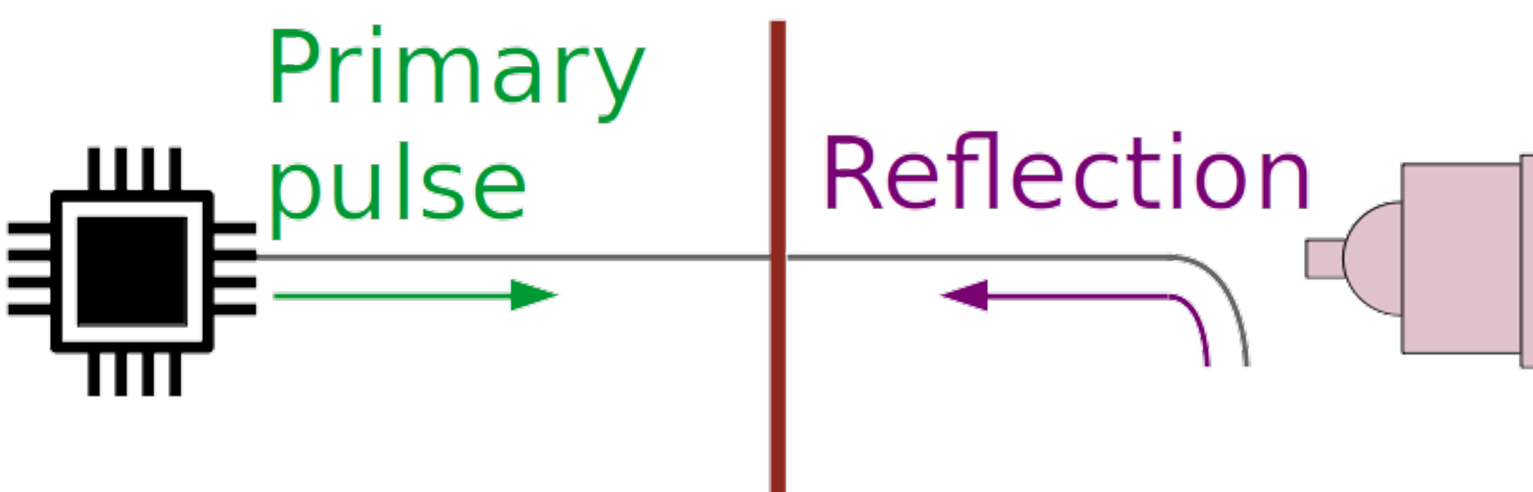
\includegraphics[width=1.1\textwidth]{commissioning/fig_commissioning/scheme_reflecto_1.pdf}
    \captionsetup{justification=centering}
    \caption{Cable not connected at PMT.
      \label{subfig:reflecto_pmt}}

  \end{subfigure}
  \hfill
  \begin{subfigure}[b]{0.3\textwidth}
    \centering
    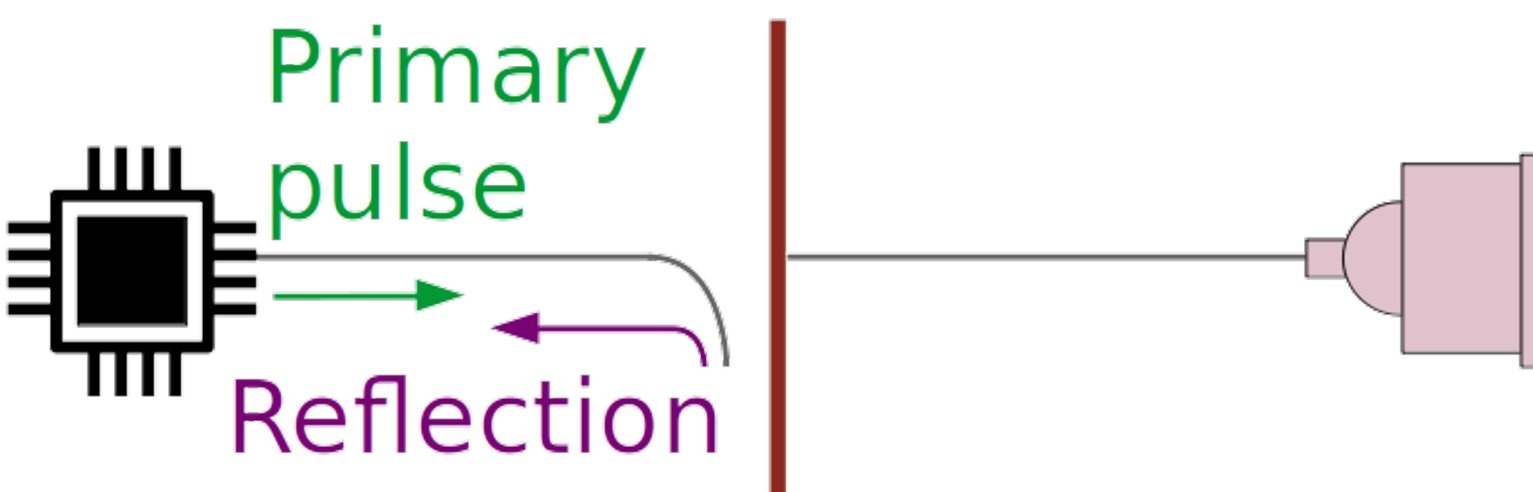
\includegraphics[width=1.1\textwidth]{commissioning/fig_commissioning/scheme_reflecto_2.pdf}
    \captionsetup{justification=centering}
    \caption{Cable not connected at patch panel.
      \label{subfig:reflecto_pp}}

  \end{subfigure}
  \caption{A representation of pulses sent in a cable for the reflectometry analysis is given.
    The electronic boards are symbolised by the black chip, and the patch panel by the red vertical bar.
    Three scenario where a primary pulse is sent in one cable (represented in grey), are represented.
    (a) The cable is well connected at the patch panel and at the PMT. The signal reflects at the PMT divider.
    (b) The cable is not connected at PMT and the signal is reflected at the end of the cable.
    (c) The cable is not connected at patch panel and the signal is reflected at the end of the external cable.\label{fig:reflecto_scheme}}

\end{figure}
Then the signal travels back from the PMT to the electronic board channel, where it is recorded by the acquisition.
We called this recorded reflected pulse \emph{secondary} pulse.
An example of the total recorded signal is displayed in Fig.~\ref{subfig:total_waveform}.
In order to accumulate enough statistics, we send thousands of pulses in each coaxial cable.
The analyses of the shape and of the arrival time of those secondary pulses for each channel is called \emph{reflectometry}, and allow us to check the coaxial cable conditions and to control their lengths.

\subsection{Pulse timing: controlling cable lengths}
\label{subsec:timing}

The first step of this analysis is to experimentally determine the length $l_{j}^{m}$ for all signal cables $j$ installed on the demonstrator.
This length is defined as
\begin{equation}
  l_{j}^{m}= 0.5\,t_{j}\,v_{p}\, ,
\end{equation}
where $t_{j}$ stands as the time made by the electrons to do a round trip between one electronic channel and one PMT, and $v_{p}$ is the velocity of electrons in the coaxial cables, which can be expressed as a fraction of light speed in vacuum, $c$.
The time difference $t_{j}$ between the primary pulse and the secondary pulse is written as
\begin{equation}
  t_{j} = \braket{t_{\text{secondary pulse}}-t_{\text{primary pulse}}}_{p} \, \text{,}
\end{equation}
$\braket{}_{p}$ being the average over all pulses sent in one single cable $j$.
The velocity $v_{p}$ is supplied by the cable manufacturer as
\begin{equation*}
  v_{p}=\frac{c}{\sqrt{\epsilon_{r}}}\,\text{,}
\end{equation*}
with $\epsilon_{r}$ the relative dielectric constant of the material.
Therefore, this celerity depends on the components.
For the coaxial cables chosen in the demonstrator design, the data sheet of the cable gives ${v_{p}=0.69\,c}$.
A study is performed to verify experimentally the value of $v_{p}$.
Three cables of different lengths are measured with a precision of $1$ cm.
A thousand of primary pulses are sent in each of the three cables, then the time for each secondary pulse is recorded.
At the end, we have three independent measures of the velocity $v_{p}$ in the used coaxial cables.
In Fig.~\ref{fig:celerity} is displayed the lengths $l_{j}$ as a function of the times $t_{j}$.
\begin{figure}[h]
  \centering
  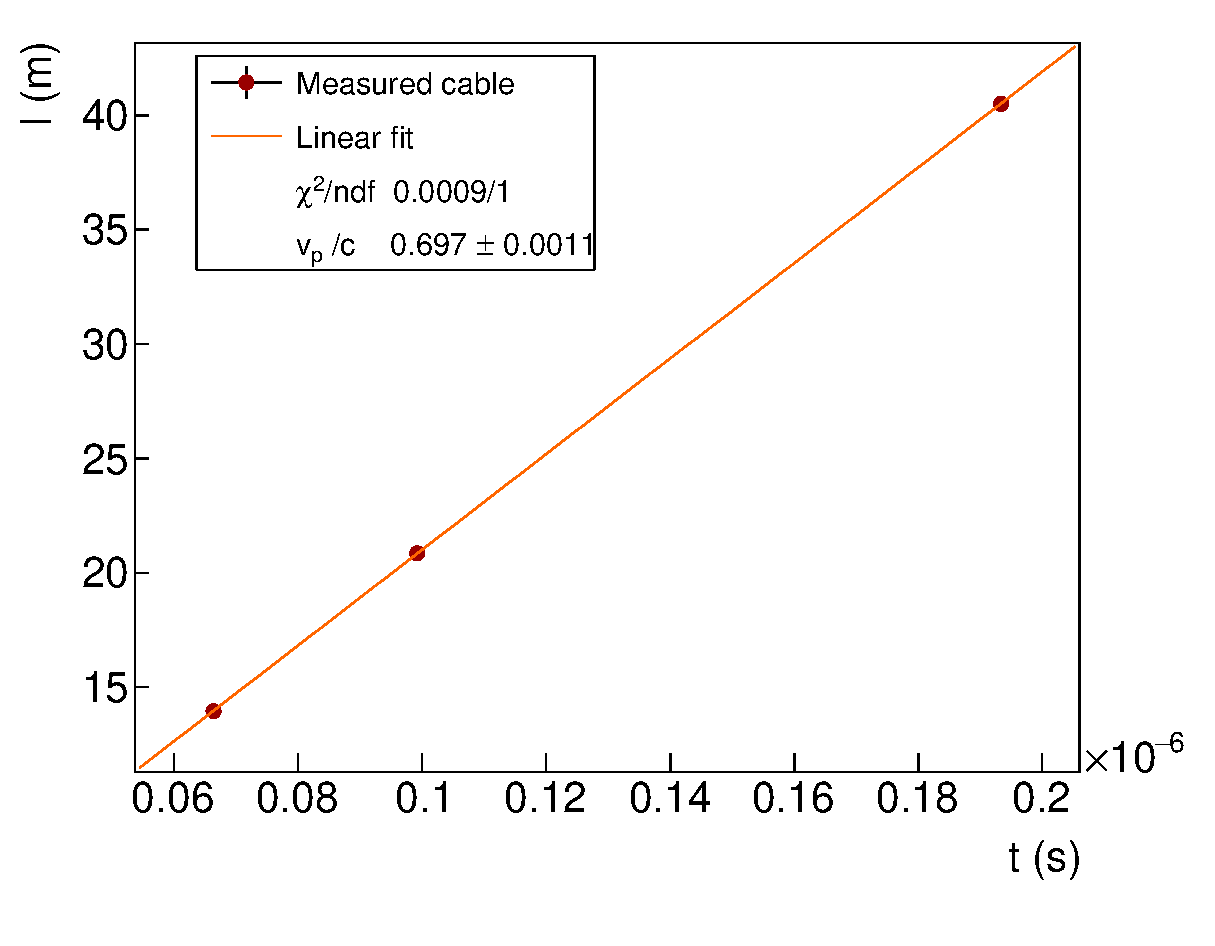
\includegraphics[width=15cm]{commissioning/fig_commissioning/celerity.eps}
  \caption{Three different lengths $l_{j}$ of cables are measured.
    Pulses are sent inside all cables.
    The lengths $l_{j}$ are plotted as a function of the time differences $t_{j}$ between primary and secondary pulses.
    The value of $v_{p}/c$ fitted from the data points is displayed.
    This value of $0.697\pm 0.0011$ shows the compatibility with the one supplied by the constructor, of $0.69$ c.
    \label{fig:celerity}}
\end{figure}
The fitted value of $v_{p}/c = 0.697\pm 0.0011$ is displayed and shows a compatibility up to $7\sigma$ with the data sheet.

As we want to determine the time interval $t_{j}$, we have to define what is the \emph{time} of a pulse.
In this analysis, we use a technique called Constant Fraction Discriminator (CFD), providing an amplitude-independent information about time of a pulse.
This algorithm aims at tracking a signal and defining its time arrival at a given fraction $f$ of its maximal amplitude.
The two main advantages of this technique is that it provides an efficient rejection of the noise in the acquisition window, and gives a good resolution on the measured time.
Nevertheless, the possible influence of the chosen value for the $f$ parameter on this time resolution has to be investigated.
We perform such a study in Sec.~\ref{subsec:CFD}.
We concluded that the highest precision on the time measurement arises for $f = 40\%$, and we adopt this value for the following analysis.
A graphic representation of the CFD time search is given in fig.~\ref{subfig:zoom_secondary}.
\begin{figure}[h]
  \centering
  \begin{subfigure}[t]{0.7\textwidth}
    \centering
    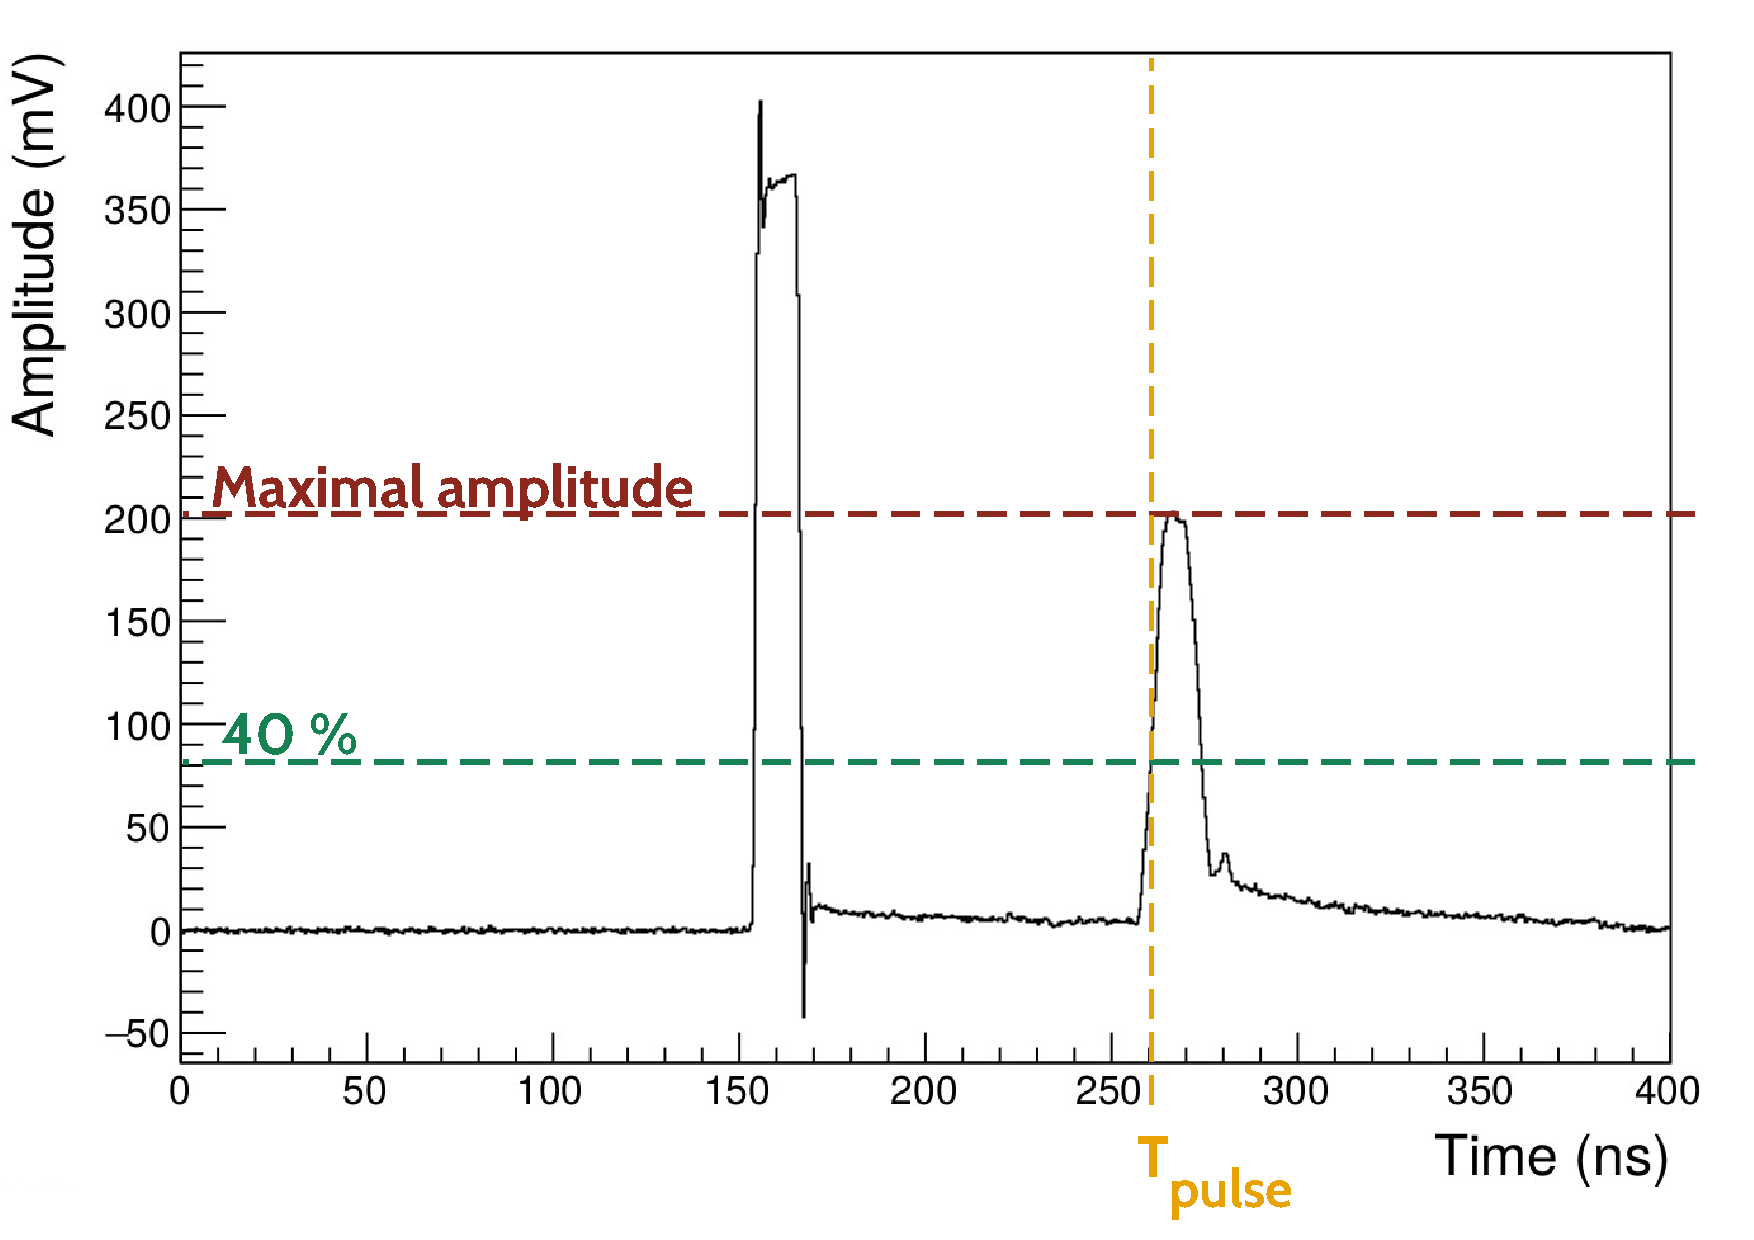
\includegraphics[trim={1.2cm 3.5cm 1.7cm 3.1cm},clip,width=1\textwidth]{commissioning/fig_commissioning/CFD_example.pdf}
    \captionsetup{justification=centering}
    \caption{Total recorded waveform
      \label{subfig:total_waveform}}
  \end{subfigure}
  \hfill
  \begin{subfigure}[t]{0.7\textwidth}
    \centering
    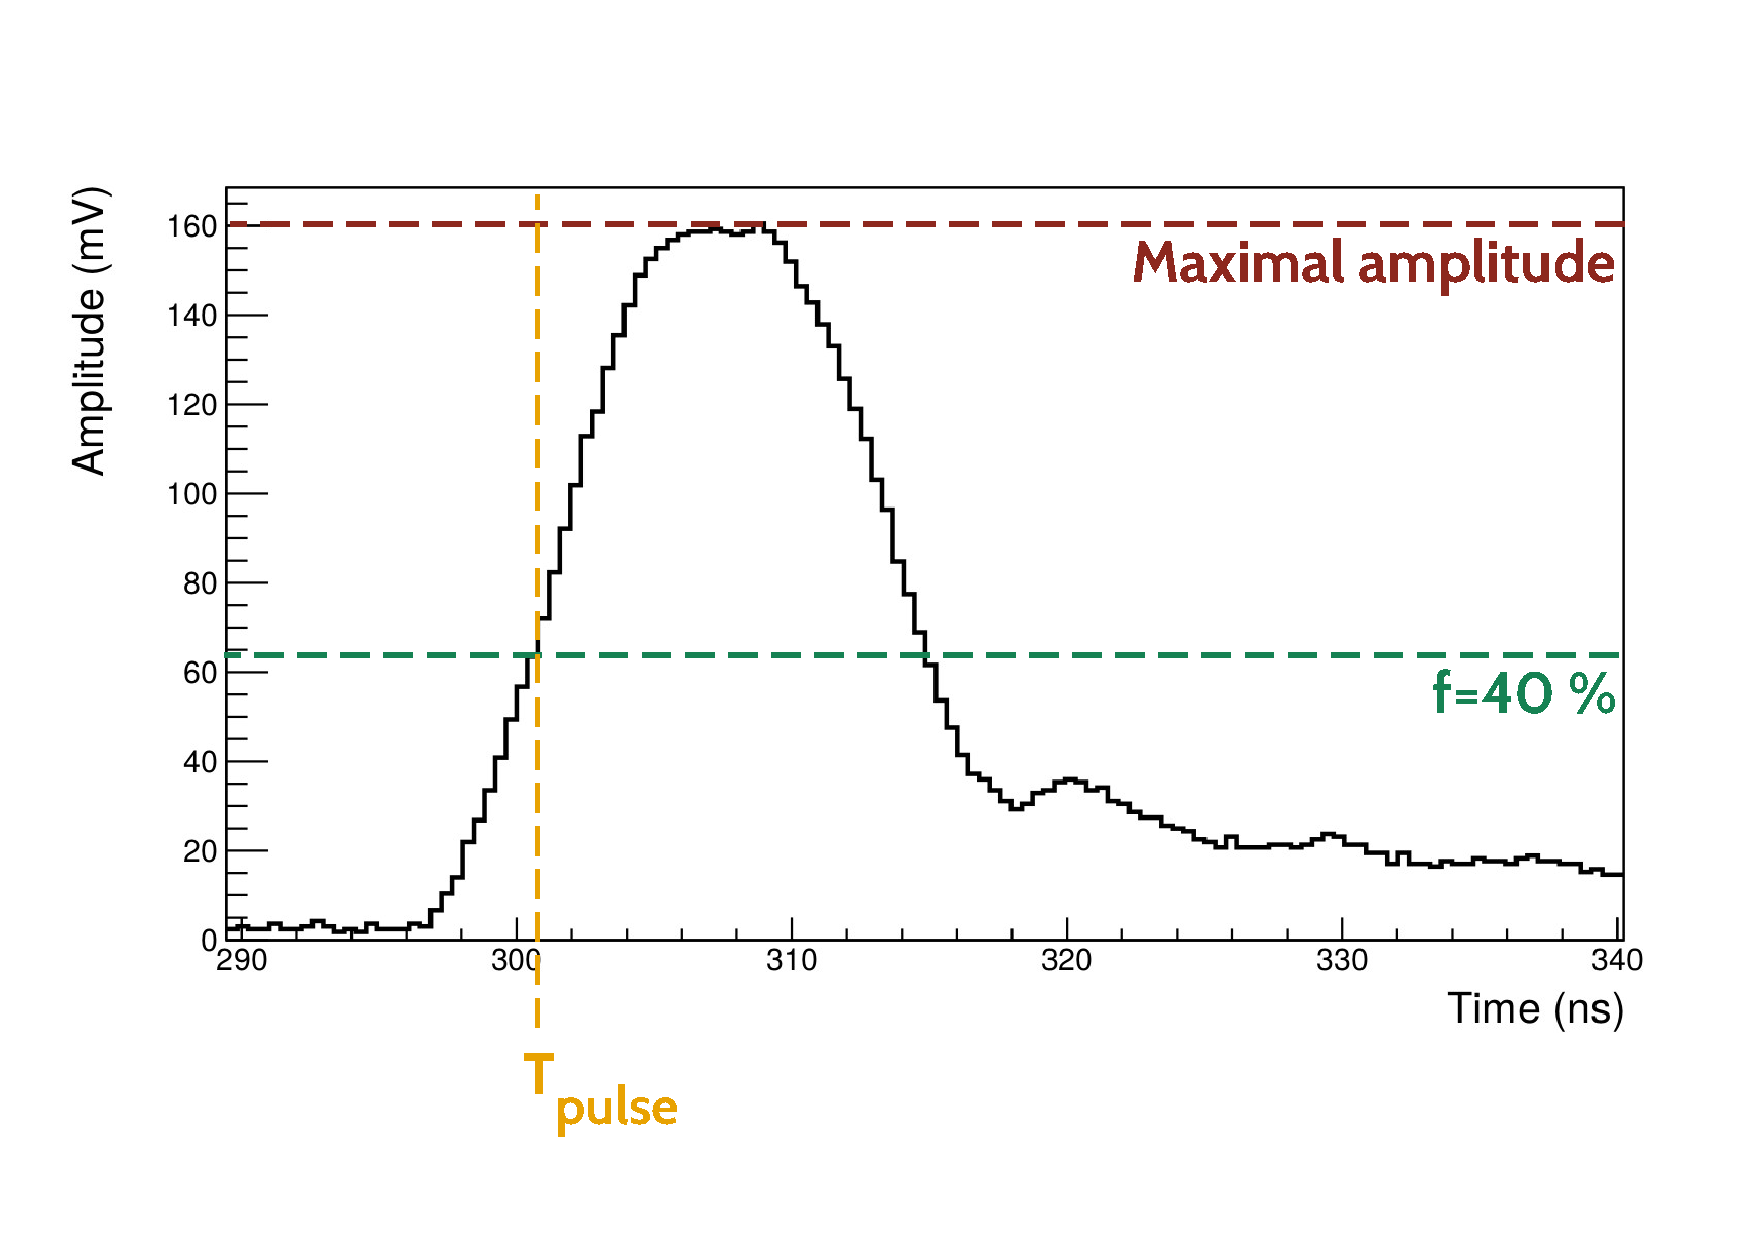
\includegraphics[trim={1.2cm 1.5cm 1.7cm 3.1cm},clip,width=1\textwidth]{commissioning/fig_commissioning/CFD_example_zoom.pdf}
    \captionsetup{justification=centering}
    \caption{Zoom on secondary pulse
      \label{subfig:zoom_secondary}}
  \end{subfigure}
  \caption{(a) Total recorded waveform: primary pulse (left) and secondary the pulse (right).
    (b) Zoom on the secondary pulse.
    A representation of time computed with a Constant Fraction Discriminator (CFD) is provided.
    Its maximal amplitude (red dotted line) and its fraction for $\text{f}=40\%$ (green dotted line) are displayed.
    The time $\text{T}_{\text{pulse}}$ (orange dotted line) represents the time of arrival of the secondary pulse computed with CFD, with the fraction $\text{f}=40\%$.
    \label{fig:CFD}}
\end{figure}
As we want to measure the installed cable lengths $l^{m}_{j}$, and compare them to the initially designed ones, $l^{d}_{j}$, we define the length difference $\Delta L_{j}$ as:
\begin{equation}
  \Delta L_{j} = l^{m}_{j}-l^{d}_{j}\, .
\end{equation}
In Fig.~\ref{fig:LengthDiff} is displayed the distribution $\Delta L$ for all the measured lengths.
\begin{figure}[h]
  \centering
  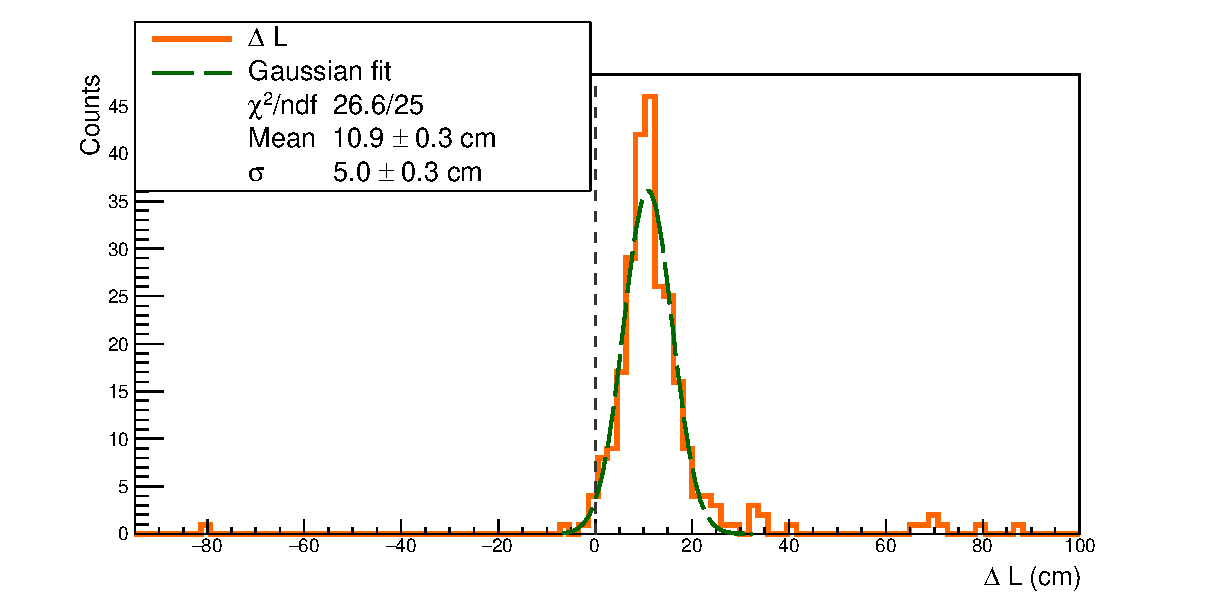
\includegraphics[width=15cm]{commissioning/fig_commissioning/length_diff.eps}

  \caption{The distribution of difference between the measured lengths $l^{m}$ and the expected lengths $l^{d}$ is displayed in orange solid line.
    The black dashed line represents the case where $l^{m}_{j} = l^{d}_{j} \;\forall j$.
    The Gaussian fit (green dashed line) presents a mean of $10.9 \pm 0.3$ cm.
    Some data points considered as outliers are beyond $3\sigma$.
    \label{fig:LengthDiff}}
\end{figure}
In hypothetical perfect conditions, all the cables should fit the design length, in other words, $l^{d}_{j} = l^{m}_{j}$.
Consequently the $\Delta L$ distribution should a peak at zero, as materialised by the black dashed line.
However, in real conditions, the measured length can be different from the designed one, leading the $\Delta L$ distribution plotted in orange solid line.
We conclude that the observed cable length $l^{m}$ differs from $l^{d}$ by $+10.9\pm 0.3$ cm, meaning that cables are longer than expected in average.
This may reveal a bias coming from the device used to cut the cables.
In fact, during cable cutting work, we noticed that the cutting device had a tendency to slip, probably leading to cables with extra lengths.
We assumed the cutting device has a given probability to slip for one meter of cable.
If this is the case, the probability for the device to give extra length should increase with the cable length.

To verify this assumption, we plot in Fig.~\ref{fig:CutBias} the length difference $\Delta L$ as a function of the initial design length $l^{d}$ (cyan).
From those data points, we compute a linear fit (orange solid line), parameterised as $y = \alpha x + \beta$, revealing that the cutting device presents two different biases.
\begin{figure}[h]
  \centering
  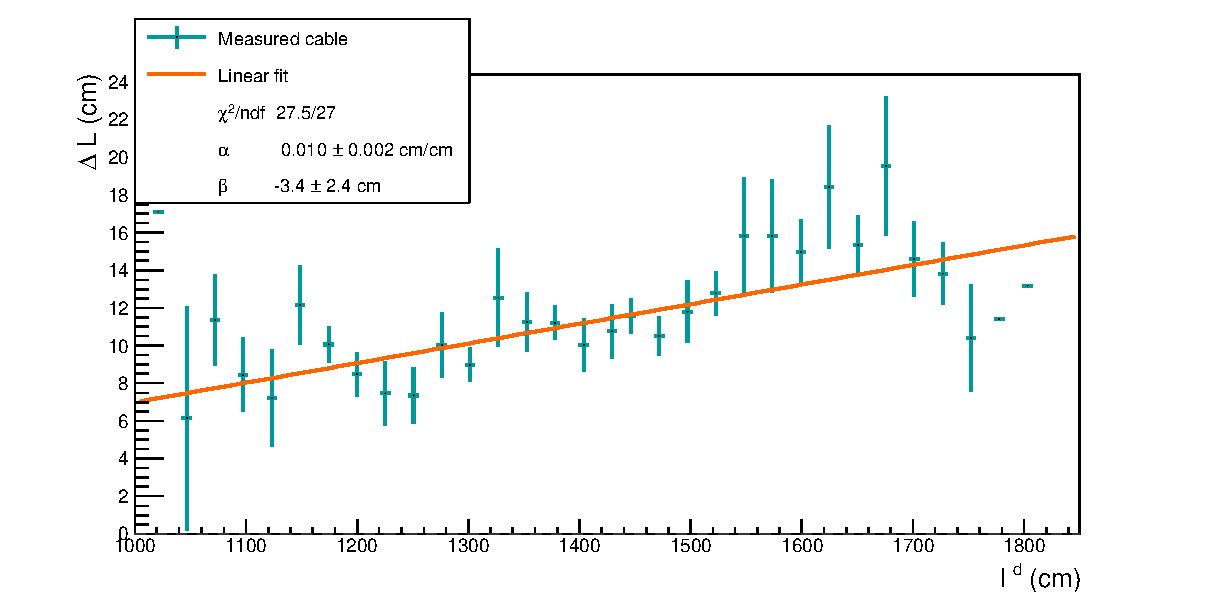
\includegraphics[width=15cm]{commissioning/fig_commissioning/cut_biais.eps}

  \caption{$\Delta L$ is plotted with $l^{d}$ (cyan), where $l^{d}$ is averaged for all the lengths designed to have the same value, being at the origin of vertical error bars.
    In black dashed line is represented the case where $l^{m} = l^{m}$.
    Data points are fitted by $\alpha x + \beta$, with $\alpha > 0$ and $\beta < 0$, revealing the two biases of the cutting device.
    \label{fig:CutBias}}
\end{figure}
The value of $\beta$ shows that the cutting device systematically took away $3.4$ cm of each cable.
Nevertheless, as the shortest cable was designed to be 10 meters long, there are no important consequences of this bias on the length difference $\Delta L$.
Besides, the slope $\alpha = 0.010\pm 0.002$ of the linear fit reveals that the cutting device adds one centimetre for every meter of cable, being compatible with the hypothesis on the cutting device sliding.
Hopefully this bias is not problematic as it makes most of the actual cable lengths longer than the design, while shorter lengths could have led to systematic connection issues to PMTs.
However, we notice that a few cables have been cut too short by mistake, the worse of them being $80$ centimetres shorter than expected.
Fortunately, this cable  was successfully connected to PMT despite this deficit.
On the contrary, few cables have a large extra length.
This probably is due to human punctual mistakes on top of the observed bias, but without any strong consequences for the calorimeter operation.
In conclusion, no important mistakes have been made when cutting cables, and we had no issue for connecting the only problematic cable.

If the main goal of this study is to check the lengths of coaxial cables, it also aims at correcting the time of recorded events, from the time made by the signal to travel from a PMT to an electronic channel.
taking into account the time for the signal to travel through cables.
This become possible with the reflectometry study we performed.
Knowing real lengths of cables and using the celerity of the signal, we deduce the time needed for the signal to travel from one given PMT divider to the electronic boards.
Then we can correct event times.

As explained previously, the time $t_{j}$ gives information about the length of the cable $j$.
We remind the coaxial cables are divided in two parts, one external and one internal, both linked by the so-called patch panel.
Thus we can use that travel time to detect possible disconnection of a cable at patch panel.
In fact, if one cable is not connected at the patch panel -- this case is illustrated in Fig.~\ref{subfig:reflecto_pp}, -- the pulse reflects at the end of the external cable part, going back to the electronic board.
This very short time, giving information about the location of the reflection, is used to tag a patch-panel disconnection.
Then, a simple check onsite can confirm this observation, and the external part of the cable can be connected to the patch panel.\\

This study allowed us to control and record the lengths of all coaxial cables installed on the SuperNEMO demonstrator at LSM, and gave information on the status of cable connections at patch panel.
We also have understood the main results on measured cable lengths and the functioning and biases of the cutting device that we used.

\subsection{Signal attenuation}
\label{subsec:attenuation}
The attenuation of an electric signal is a problem common to all electronic fields, and comes from the charge loss of an electromagnetic wave travelling in a medium.
%% Then, another test for controlling the cable condition is to check if this attenuation matches
%% the expectations (i.e. the attenuation per metre of cable given by constructor).
%% The signal attenuation car be define in two different ways:
%% \begin{itemize*}
%% \item using the signal amplitude ratio
%% \end{itemize*}
For a coaxial cable, this attenuation mainly depends on the signal frequency $f$ in MHz and on the cable characteristics.
For the coaxial cables, the theoretical linear attenuation $\alpha_{\text{att}}^{\text{th}}$, so be it the attenuation by metre of cable in dB/m, is supplied by the constructor as
\begin{equation}
  \alpha_{\text{att}}^{\text{th}} = f\sqrt{\epsilon}(\frac{a}{\sqrt{f}}+b)\,,
\end{equation}
where the factor $a$ depends on the diameter of the dielectric material on one side, and of the diameter of the conductor material on the other side, and where $b$ is function of the dielectric loss factor, characterising the material's dissipation of electromagnetic energy.
For the used coaxial cables, and with a frequency $f$ of few GHz for the signal pulses sent in cables, we calculate this attenuation as $\alpha_{\text{att}}^{\text{th}} = 1.22$ dB/m.
In a more general manner, the attenuation of a signal in dB is defined with the decimal logarithm of a power ratio.
We use this definition to determine the attenuation in the framework of the reflectometry analysis, defining the attenuation $\mathcal{A}$, for a given length of cable $l$, as
\begin{equation}
  \mathcal{A}=10\log_{10}\frac{V_{\text{primary pulse}}}{V_{\text{secondary pulse}}} \,\text{,}
\end{equation}
where $V_{i}$ is a quantity representing the intensity of the signal.
$V$ can correspond to the maximal amplitude of the pulse, as well as the \emph{integrated charge} of the pulse, defined as the amount of current received by the acquisition over a given time window.
As the provided data sheet does not specify the attenuation of which quantity (amplitude or charge) represents $\alpha_{\text{att}}^{\text{th}}$, we decide to investigate both in the following.
Then, we define the linear attenuation $\alpha_{\text{att}}^{\text{R}}$, measured by reflectometry in dB/m, with
\begin{equation}
  \mathcal{A} = f_{r}+\alpha_{\text{att}}^{\text{R}}\,l\,,
\end{equation}
with $f_{r} = -10\log_{10}R$, where $R$ is the reflection factor characterising the pulse reflection on the PMT divider.
In fact, as the circuit is opened, the pulse is reflected at the PMT divider, but only partially.
A part of the signal is not reflected but lost through the divider.
This reflection is characterised by $R$, which is function of the impedance $Z_{c}$ of the cable, and of the impedance $Z_{d}$ at the divider level, where the pulse is reflected.
It is written as
\begin{equation}
  R = \frac{Z_{d}-Z_{c}}{Z_{d}+Z_{c}}\,,
\end{equation}
where we have the limit
\begin{equation}
  \lim_{Z_{d} \to \infty} f_{r} = 0 \text{ and } R=1\,,
\end{equation}
expressing a total reflection occurring when the impedance at the PMT divider is infinite.
The main goal here is to determine the value of $\alpha_{\text{att}}^{\text{R}}$, using the reflectometry data, and to compare it with $\alpha_{\text{att}}^{\text{th}}$.
Moreover, the impedance $Z_{d}$ value at PMT divider can be estimated from the determination of $f_{r}$.
In Fig.~\ref{fig:attenuation} is shown the linear dependence between the attenuation $\mathcal{A}$ and the cable length $l$, and two data set are presented.
The cyan scattered markers represent the attenuation calculated from the amplitude ratio $A_{\text{primary pulse}}/A_{\text{secondary pulse}}$, and the magenta markers correspond to the attenuation calculated from the charge ratio $Q_{\text{primary pulse}}/Q_{\text{secondary pulse}}$.
The amplitude $A_{i}$ is given in mV and the charge $Q_{i}$ in mV.ns.
\begin{figure}[h]
  \centering
  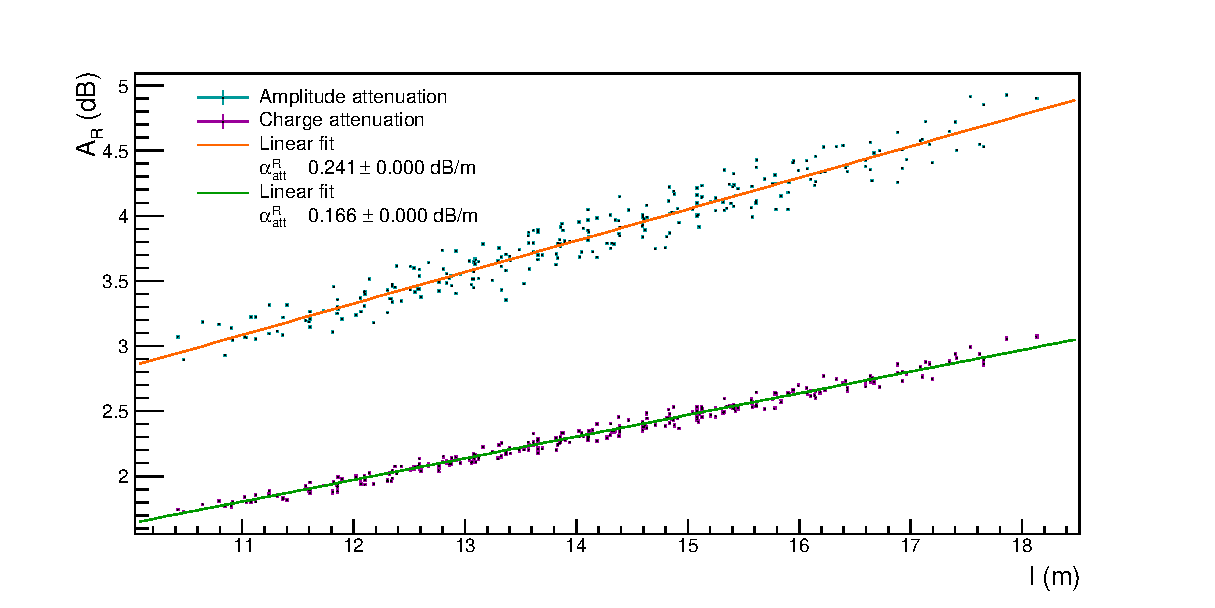
\includegraphics[width=15cm]{commissioning/fig_commissioning/attenuation_length.eps}
  \caption{The amplitude $\mathcal{A}$ is displayed as a function of the measured cable length $l$.
    The data set calculated with the amplitude (charge) is given in cyan (magenta) and fitted by a linear function in orange (green).
    The values of the slope, which represent the linear attenuation of the coaxial cables in dB/m, are respectively $\alpha_{\text{att}}^{\text{R, amp}} = 0.241\pm 0.000$dB/m and $\alpha_{\text{att}}^{\text{R, ch}} = 0.166\pm0.000$dB/m.
    The two $y$-intercept values, which represent the reflection of the pulse on the PMT divider, are $f_{r}^{amp} = 0.402\pm 0.032$ dB and $f_{r}^{ch} = -0.020\pm 0.013$ dB.
    \label{fig:attenuation}}
\end{figure}
The values of $\alpha_{\text{att}}^{\text{R}}$ and $f_{r}$, for both amplitude and charge cases, are displayed in the legend.
Firstly, the two linear fits reveal that, whether calculated with the amplitude, or with the charge, the linear attenuation $\alpha_{\text{att}}^{\text{R}}$ is smaller than the calculated one $\alpha_{\text{att}}^{\text{th}}$ (for the amplitude case, $\alpha_{\text{att}}^{\text{th}}\simeq 5\times \alpha_{\text{att}}^{\text{R, amp}}$, and for the charge case $\alpha_{\text{att}}^{\text{th}}\simeq 7\times \alpha_{\text{att}}^{\text{R, ch}}$).
That means the signal is less affected, when transmitted by the cable, than expected.
Secondly, the attenuation in charge is less important that the attenuation in amplitude.
This can be easily explained: as it is integrated over time, the charge is a quantity less affected by amplitude variations that the amplitude itself.
For the same reason, the charge data set points are less spread than the amplitude ones, meaning that we are less sensitive to cable length variations when using the charge quantity.


This work achieved, we want to verify if no cable was damaged after installation.
Reflectometry also aimed at checking cable conditions by performing waveform shape analysis on secondary pulses.

\subsection{Pulse shape analysis}
\label{subsec:pulse_shape}
In Fig.~\ref{fig:CFD} is displayed an example of \emph{normal} pulse, which corresponds to the case represented in Fig.~\ref{subfig:reflecto_normal}.
In this case, the pulse sent in the cable travels to the PMT, and goes back to the acquisition after reflection on the divider.


\subsection{Comparison with $^{60}$Co}

\subsection{Conclusion}
A faire : regarder le rising time en fonction de la longueur du cable\\
Regarder la différence de temps de montée du signal sur deux PMs très éloignés

\section{Calibrating the electronic boards}
\label{sec:TimeSynchroFEB}

\subsection{Principle}
\subsection{Measuring the time offset of front end boards}
\subsection{Results}


\section{Energy calibration of optical modules}
\label{sec:comm_energy_calibration}


*thèse Arnaud page 103*

As described in Sec.~\ref{subsec:OMtimeResponse}, the collected charge at PM voltage divider is proportional to the amount of incident photoelectrons, and then to the initially deposited energy inside the scintillator.
Once optical modules were assembled (optical coupling, packing, shielding integration), they were individually tested at Bordeaux laboratory, CENBG, with an electron spectrometer [ref].
Their energy resolutions for $1$ MeV-electrons at the centre of scintillator front face were determined.
High voltages were set to optimal values, to obtain an amplitude of $300$ mV for $1$ MeV electrons.
However, after calorimeter integration, due to different environment, amplitude spectra of each optical block have to be re-aligned.
This work was performed by Axel Pin, PhD student at CENBG.
We give in this section a summary of this energy calibration study.

*A finir\\




\section{Baseline studies}
\label{sec:comm_baseline}

\section{Light Injection System}
\label{sec:LI}

\include{theory/theory}
\chapter*{Conclusion}
\addcontentsline{toc}{chapter}{Conclusion}


\bibliographystyle{unsrt}
\bibliography{bibliography_thesis}

\end{document}
